\documentclass[12pt, a4paper, onecolumn, oneside]{report}
\usepackage[bahasa]{babel}
\addto\captionsbahasa{\renewcommand{\bibname}{DAFTAR PUSTAKA}} % PERINTAH BARU
\usepackage[top=3cm, left=4cm, bottom=3cm, right=3cm]{geometry}
\usepackage{graphicx}
\usepackage{float} % untuk posisi [H] yang lebih baik
\usepackage{titlesec}
\usepackage{chngcntr}
\usepackage{tocbasic}
\usepackage{tocloft}
\usepackage{setspace}
\usepackage{needspace}
\usepackage{longtable}
\usepackage{times}
\usepackage{booktabs}
\usepackage[table]{xcolor}
\usepackage{multirow}
\usepackage{pdflscape}
\usepackage{pdfpages}


% \bibliographystyle{ieeetr}
% \bibliographystyle{IEEEtran}
\usepackage[natbibapa]{apacite}
\bibliographystyle{apacite-dkk}
\renewcommand{\BOthers}[1]{dkk.\hbox{}}
\renewcommand{\BOthersPeriod}[1]{dkk.\hbox{}}

\usepackage[utf8]{inputenc}
\usepackage{tikz}
\usetikzlibrary{shapes, arrows.meta, positioning, fit, backgrounds, calc}

\usepackage{tabularx}
\usepackage{array}
\usepackage{amsmath}
\usepackage{amssymb}
\usepackage{url}
\usepackage{indentfirst}
\usepackage[hidelinks]{hyperref}

% Pengaturan format bab
\renewcommand{\thechapter}{\Roman{chapter}}
\titleformat{\chapter}[display]
{\bfseries\centering\large}
{\MakeUppercase{\chaptertitlename} \thechapter}
{0pt}
{\MakeUppercase}
\titleformat{name=\chapter,numberless}[display]
{\bfseries\centering\large}
{}
{0pt}
{\MakeUppercase}
\titlespacing*{\chapter}{0pt}{-30pt}{20pt}

% Pengaturan format section
\renewcommand{\thesection}{\arabic{chapter}.\arabic{section}}
\renewcommand{\thesubsection}{\arabic{chapter}.\arabic{section}.\arabic{subsection}}
\titleformat{\section}
{\bfseries}
{\thesection}{1em}{}

% Pengaturan format subsection
\titleformat{\subsection}
{\bfseries}
{\thesubsection}{1em}{}

% Pengaturan spasi
\onehalfspacing

% Mengurangi Overfull \hbox kecil (pemenggalan baris)
\emergencystretch=2em

% Pengaturan penomoran
\counterwithin{figure}{chapter}
\counterwithin{table}{chapter}
\counterwithin{equation}{chapter}
\renewcommand{\thefigure}{\arabic{chapter}.\arabic{figure}}
\renewcommand{\thetable}{\arabic{chapter}.\arabic{table}}
\renewcommand{\theequation}{\arabic{chapter}.\arabic{equation}}
\renewcommand{\cftfigpresnum}{Gambar~}
\renewcommand{\cfttabpresnum}{Tabel~}
\settowidth{\cftfignumwidth}{Gambar~10.10\quad}
\settowidth{\cfttabnumwidth}{Tabel~10.10\quad}

\renewcommand{\cftchappresnum}{BAB }
\setlength{\cftchapnumwidth}{5em}
\renewcommand{\cftchapaftersnum}{}  % jika ingin titik setelah nomor

% \renewcommand{\bibname}{DAFTAR PUSTAKA}

\makeatletter
\renewcommand{\tableofcontents}{%
  \@starttoc{toc}%
}
\renewcommand{\listoffigures}{%
  \@starttoc{lof}%
}
\renewcommand{\listoftables}{%
  \@starttoc{lot}%
}
\makeatother

% Pastikan nama-nama tersebut sesuai (dalam huruf besar)
\renewcommand{\contentsname}{DAFTAR ISI}
\renewcommand{\listfigurename}{DAFTAR GAMBAR}
\renewcommand{\listtablename}{DAFTAR TABEL}

% Memuat variabel dari metadata.tex
% ============================================
% metadata.tex
% Berisi definisi semua variabel untuk dokumen usulan penelitian S3
% ============================================

% Jenis dokumen
% \newcommand{\jenisdokumen}{USULAN PENELITIAN S3}
\newcommand{\jenisdokumen}{UJIAN KOMPREHENSIF}
% \newcommand{\jenisdokumen}{UJIAN KOMPREHENSIF}

% Judul penelitian
\newcommand{\judul}{\MakeUppercase{Adaptasi CDE-Mapper Pemetaan Terminologi Klinis untuk Teks Bahasa Indonesia: Pendekatan Berbasis LLM dan Hybrid Retrieval}}

% Penulis dan NIM
\newcommand{\penulis}{Anie Rose Irawati}
\newcommand{\nim}{24/551784/SPA/01084}

% Program studi, departemen, fakultas, universitas
\newcommand{\programstudi}{S3 Ilmu Komputer}
\newcommand{\departemen}{Departemen Ilmu Komputer dan Elektronika}
\newcommand{\fakultas}{Fakultas Matematika dan Ilmu Pengetahuan Alam}
\newcommand{\universitas}{Universitas Gadjah Mada}

% Tanggal sidang/pengesahan
\newcommand{\tanggal}{.......... 2026}

% Dewan penguji (gunakan placeholder jika belum diisi)
\newcommand{\ketuaPenguji}{...............}   % masih kosong
\newcommand{\promotor}{Afiahayati, S.Kom., M.Cs., Ph.D}
\newcommand{\kopromotor}{Dr. Lukman Heryawan, S.T., M.T.}
\newcommand{\pengujiSatu}{Prof Dr. XYZ, M.SC}   % placeholder
\newcommand{\pengujiDua}{Prof Dr. ABC, M.SC}    % placeholder
\newcommand{\pengujiTiga}{Prof Dr. XYZ, M.SC}   % placeholder (penguji tambahan)

\begin{document}

% Halaman Judul
\begin{titlepage}
    \centering
    \vspace*{0.5cm}
    
    {\bfseries\large \jenisdokumen\par}
    \vspace{1.3cm}
    
    {\bfseries\large \judul\par}
    \vspace{1.3cm}
    
    
\includegraphics[width=2in, height=2in]{media/logo-ugm.png}
    \vspace{1.3cm}
    
    {\bfseries Diusulkan Oleh:\par}
    {\bfseries \penulis\par}
    \vspace{1cm}
    
    {\bfseries Dosen Pembimbing:\par}
    {\bfseries \promotor\par}
    {\bfseries \kopromotor\par}
    \vspace{1.3cm}
    
    {\bfseries PROGRAM DOKTOR ILMU KOMPUTER\par}
    {\bfseries DEPARTEMEN ILMU KOMPUTER DAN ELEKTRONIKA\par}
    {\bfseries FAKULTAS MATEMATIKA DAN ILMU PENGETAHUAN ALAM\par}
    {\bfseries UNIVERSITAS GADJAH MADA\par}
    {\bfseries YOGYAKARTA\par}
    {\bfseries 2026\par}
\end{titlepage}

% Halaman Pengesahan
\newpage
\pagenumbering{roman}
\begin{sloppypar}
% % ============================================
% main.tex
% File utama yang memanggil metadata.tex dan menyusun halaman pengesahan
% ============================================

\begin{center}
    \vspace*{0.2cm}
    
    \textbf{\large HALAMAN PERSETUJUAN}
    
    \vspace{0.8cm}
    
    \textbf{\large \jenisdokumen} \\

    \vspace{0.8cm}

    % Program Studi \programstudi, \departemen, \fakultas, \universitas \\
    
    \vspace{0.8cm}
    
    \textbf{\large \judul}
    
    \vspace{0.8cm}
    
    Disusun Oleh:\\
    \vspace{0.5cm}
    \textbf{\penulis} \\
    \textbf{\nim}
       
    \vspace{0.5cm}
    
    
    Yogyakarta, \tanggal \\
    Menyetujui,
    
    \vspace{2.5cm}
    
    \begin{center}
    {\renewcommand{\arraystretch}{0.7}%
    \begin{tabular}{>{\centering\arraybackslash}p{7.2cm}>{\centering\arraybackslash}p{7.2cm}}
        \underline{\promotor} & \underline{\kopromotor} \\
        \textbf{Promotor} & \textbf{Ko-Promotor} \\[2.2cm]
    
    \end{tabular}}
    \end{center}

    
\end{center}
% % ============================================
% main.tex
% File utama yang memanggil metadata.tex dan menyusun halaman pengesahan
% ============================================

\begin{center}
    \vspace*{0.2cm}
    
    \textbf{\large HALAMAN PENGESAHAN}
    
    \vspace{0.8cm}
    
    \textbf{\large \jenisdokumen}
    
    \vspace{0.8cm}
    
    \textbf{\large \judul}
    
    \vspace{0.8cm}
    
    
    \textbf{\penulis} \\
    \textbf{\nim}
       
    \vspace{0.5cm}
    
    Dipertahankan dihadapan Dewan Penguji Program Studi \programstudi \\
    \departemen \\
    \fakultas \\
    \universitas
    
    \vspace{0.5cm}
    
    Pada Tanggal \tanggal
    
    \vspace{1.6cm}
    {\renewcommand{\arraystretch}{0.7}%
    \begin{tabular}{c}
        \underline{\ketuaPenguji} \\
        \textbf{Ketua Penguji}
    \end{tabular}}
    
    \vspace{2cm}

    {\renewcommand{\arraystretch}{0.9}%
    \begin{tabular}{>{\raggedright\arraybackslash}p{7.2cm}>{\raggedright\arraybackslash}p{7.2cm}}
        \underline{\promotor} & \underline{\pengujiSatu} \\
        Promotor & Penguji \\[1.7cm]
        \underline{\kopromotor} & \underline{\pengujiDua} \\
        Ko-Promotor & Penguji \\[1.7cm]
        & \underline{\pengujiTiga} \\
        & Penguji \\
    \end{tabular}}
\end{center}
\includepdf[pages=-]{build-signature-review/persetujuan-flat-test.pdf}
\end{sloppypar}
\newpage


% Daftar Isi
\chapter*{DAFTAR ISI}
\addcontentsline{toc}{chapter}{DAFTAR ISI}
\makeatletter\@starttoc{toc}\makeatother

\newpage

% Daftar Gambar
\chapter*{DAFTAR GAMBAR}
\addcontentsline{toc}{chapter}{DAFTAR GAMBAR}
\makeatletter\@starttoc{lof}\makeatother

\newpage

\chapter*{DAFTAR TABEL}
\addcontentsline{toc}{chapter}{DAFTAR TABEL}
\makeatletter\@starttoc{lot}\makeatother
\newpage
\chapter*{DAFTAR ISTILAH}
\addcontentsline{toc}{chapter}{DAFTAR ISTILAH}

{\setstretch{1}
\setlength{\parskip}{0pt}
\begin{description}
\setlength{\itemsep}{0.75\baselineskip}
\setlength{\parsep}{0pt}
\setlength{\topsep}{0pt}

    \item[\textit{Ablation study}] Teknik evaluasi untuk mengukur kontribusi setiap komponen model dengan cara menghapus atau menonaktifkan komponen tertentu secara bertahap.

    \item[AI (\textit{Artificial Intelligence})] Cabang ilmu komputer yang mengembangkan sistem untuk meniru kemampuan kognitif manusia, termasuk pemahaman bahasa dan pengambilan keputusan.

    \item[\textit{Baseline}] Metode atau model pembanding yang digunakan sebagai acuan untuk menilai peningkatan kinerja pendekatan yang diusulkan.

    \item[BERT] \textit{Bidirectional Encoder Representations from Transformers}, model bahasa berbasis transformer dua arah untuk memahami konteks kata berdasarkan hubungan dengan kata sebelum dan sesudahnya.

    \item[BiLSTM] \textit{Bidirectional Long Short-Term Memory}, jenis RNN yang memproses urutan teks dari dua arah (kiri dan kanan); sering digunakan untuk NER sebelum era transformer.

    \item[BioNER] \textit{Biomedical Named Entity Recognition}, teknik untuk mengenali dan mengekstraksi entitas penting pada teks biomedis atau klinis, seperti penyakit, obat, gejala, dan prosedur.

    \item[CDE (\textit{Common Data Element})] Elemen data standar yang digunakan untuk menyeragamkan definisi, struktur, dan representasi data agar dapat digunakan lintas sistem.

    \item[CDE-Mapper] \textit{Framework} pemetaan yang dirancang untuk menghubungkan elemen data atau istilah ke kosakata terkendali; menjadi dasar adaptasi model dalam penelitian ini.

    \item[CDSS (\textit{Clinical Decision Support System})] Sistem yang membantu tenaga kesehatan dalam pengambilan keputusan klinis melalui penyediaan rekomendasi, peringatan, atau informasi yang relevan.

    \item[Code-Mixing] Fenomena pencampuran dua bahasa dalam satu ujaran atau teks; dalam konteks klinis Indonesia, sering mencampur istilah Indonesia dengan Inggris.

    \item[\textit{Controlled vocabulary}] Kosakata terkendali berupa himpunan istilah standar yang digunakan secara konsisten agar representasi data memiliki makna yang seragam.

    \item[\textit{Coverage}] Metrik evaluasi yang menunjukkan sejauh mana sistem mampu menghasilkan pemetaan untuk data atau istilah yang diuji.

    \item[CRF (\textit{Conditional Random Field})] Lapisan probabilistik yang sering ditambahkan di atas BiLSTM atau BERT untuk memastikan konsistensi label berurutan dalam tugas NER.

    \item[cTAKES] \textit{clinical Text Analysis and Knowledge Extraction System}, toolkit NLP \textit{open-source} dari Mayo Clinic untuk ekstraksi entitas klinis dari teks rekam medis.

    \item[\textit{Deep learning}] Pendekatan pembelajaran mesin berbasis jaringan saraf berlapis banyak yang mampu mempelajari representasi data yang kompleks.

    \item[EHR (\textit{Electronic Health Record})] Rekam kesehatan elektronik yang menyimpan riwayat informasi kesehatan pasien secara digital dan dapat diakses lintas layanan.

    \item[\textit{Ensemble retrieval}] Strategi pencarian kandidat yang menggabungkan beberapa \textit{retriever} secara paralel (misal SPLADE dan SapBERT) untuk menghasilkan daftar kandidat yang lebih kaya.

    \item[F1-score] Metrik evaluasi yang menggabungkan \textit{precision} dan \textit{recall} untuk menilai keseimbangan antara ketepatan dan kelengkapan hasil model.

    \item[FHIR (\textit{Fast Healthcare Interoperability Resources})] Standar pertukaran data kesehatan yang dikembangkan oleh HL7 untuk mendukung interoperabilitas sistem kesehatan secara digital.

    \item[\textit{Framework}] Kerangka kerja konseptual dan teknis yang memandu perancangan, integrasi, dan implementasi komponen dalam suatu sistem.

    \item[\textit{Gold standard}] Data acuan yang telah diverifikasi, umumnya oleh pakar, dan digunakan sebagai rujukan utama dalam pelatihan, pengujian, atau validasi sistem.

    \item[GPT (\textit{Generative Pre-trained Transformer})] Model bahasa generatif berbasis transformer yang dilatih terlebih dahulu pada korpus besar untuk menghasilkan dan memahami teks.

    \item[\textit{Graph embeddings}] Teknik representasi simpul atau entitas dalam graf ke dalam bentuk vektor numerik agar hubungan semantik dapat diproses oleh model komputasional.

    \item[HL7 (\textit{Health Level Seven})] Organisasi pengembang standar pertukaran data kesehatan, termasuk FHIR.

    \item[ICD (\textit{International Classification of Diseases})] Sistem klasifikasi penyakit yang digunakan untuk pengodean diagnosis, pelaporan statistik, dan manajemen kesehatan.

    \item[ICD-10] Revisi kesepuluh dari \textit{International Classification of Diseases} yang banyak digunakan untuk klasifikasi diagnosis dan kondisi kesehatan.

    \item[\textit{Inter-Annotator Agreement}] Tingkat kesepakatan antara dua atau lebih anotator dalam memberikan label pada dataset; diukur dengan koefisien Kappa.

    \item[\textit{Interoperabilitas}] Kemampuan dua atau lebih sistem untuk bertukar data dan memanfaatkan data tersebut secara efektif dalam konteks yang sama.

    \item[\textit{Knowledge graph}] Representasi pengetahuan dalam bentuk graf yang memodelkan entitas dan relasinya untuk mendukung penelusuran serta penalaran semantik.

    \item[\textit{Knowledge reservoir}] Basis penyimpanan pasangan label--kode yang telah tervalidasi untuk mempercepat inferensi dan meningkatkan konsistensi lintas dokumen.

    \item[KPTL] Kode Pembiayaan Tindakan dan Layanan Kesehatan Nasional, terminologi nasional Indonesia untuk kebutuhan pembiayaan kesehatan.

    \item[LLaMA (\textit{Large Language Model Meta AI})] Keluarga model bahasa besar terbuka dari Meta (7B--65B parameter) yang dioptimalkan untuk efisiensi inferensi.

    \item[LLM (\textit{Large Language Model})] Model bahasa berukuran besar dengan miliaran parameter, mampu memahami, merangkum, dan menghasilkan teks secara kontekstual.

    \item[LOINC (\textit{Logical Observation Identifiers Names and Codes})] Standar terminologi untuk observasi klinis, pemeriksaan laboratorium, dan pengukuran kesehatan.

    \item[\textit{Low-resource language}] Bahasa dengan sumber daya data, korpus, dan anotasi digital yang terbatas untuk pengembangan model komputasional.

    \item[\textit{Machine learning}] Pendekatan komputasional yang memungkinkan sistem mempelajari pola dari data untuk membuat prediksi atau keputusan tanpa diprogram secara eksplisit.

    \item[MRR (\textit{Mean Reciprocal Rank})] Metrik evaluasi \textit{retrieval} yang memberi bobot lebih tinggi jika kandidat benar muncul pada peringkat lebih awal.

    \item[NER (\textit{Named Entity Recognition})] Teknik NLP untuk mengidentifikasi dan mengklasifikasikan entitas penting dalam teks.

    \item[NLP (\textit{Natural Language Processing})] Bidang kecerdasan artifisial yang berfokus pada pengolahan, analisis, dan pemahaman bahasa manusia oleh komputer.

    \item[OMOP CDM] \textit{Observational Medical Outcomes Partnership Common Data Model}, model data standar untuk standardisasi struktur data observasional kesehatan.

    \item[\textit{Ontologi}] Representasi formal mengenai konsep-konsep dalam suatu domain beserta relasi antarkonsep untuk mendukung konsistensi makna.

    \item[\textit{Post-coordination}] Kemampuan membuat konsep baru dalam SNOMED CT dengan menggabungkan beberapa konsep yang sudah ada beserta relasinya.

    \item[\textit{Precision}] Metrik evaluasi yang menunjukkan proporsi hasil prediksi yang benar dari seluruh hasil yang diprediksi positif atau relevan oleh sistem.

    \item[\textit{Preprocessing}] Tahap pembersihan dan normalisasi teks sebelum pemrosesan lebih lanjut (\textit{case folding}, \textit{stemming}, normalisasi singkatan, dll.).

    \item[\textit{Query decomposition}] Tahap pemecahan CDE komposit menjadi komponen-komponen kecil (\textit{base entity}, \textit{domain}, \textit{unit}, \textit{visit}, dll.) menggunakan LLM.

    \item[RAG (\textit{Retrieval-Augmented Generation})] Pendekatan yang menggabungkan pencarian informasi dengan generasi teks berbasis model bahasa untuk meningkatkan relevansi keluaran.

    \item[\textit{Recall}] Metrik evaluasi yang menunjukkan proporsi data relevan yang berhasil ditemukan atau dipetakan dengan benar oleh sistem.

    \item[Reranking] Proses mengurutkan ulang kandidat hasil \textit{retrieval} menggunakan model atau kriteria tambahan agar hasil teratas menjadi lebih relevan.

    \item[RME (Rekam Medis Elektronik)] Istilah Bahasa Indonesia untuk \textit{Electronic Health Record} (EHR) atau sistem pencatatan medis pasien secara digital.

    \item[\textit{Rule-based}] Pendekatan berbasis aturan eksplisit yang disusun secara manual untuk mengenali pola, istilah, atau relasi tertentu dalam data.

    \item[SapBERT] \textit{Retriever dense} berbasis BERT yang dirancang khusus untuk entitas biomedis, mampu mendekatkan representasi sinonim.

    \item[SATUSEHAT] Platform interoperabilitas data kesehatan nasional di Indonesia yang mengintegrasikan data antar fasilitas dan sistem kesehatan.

    \item[\textit{Self-consistency}] Mekanisme pengulangan penilaian LLM beberapa kali dengan \textit{prompt} yang sama untuk menghitung \textit{confidence score} dari hasil yang konsisten.

    \item[\textit{Semantic retrieval}] Teknik penelusuran informasi yang memanfaatkan kemiripan makna, bukan hanya kecocokan kata, untuk menemukan kandidat yang relevan.

    \item[\textit{Sentence transformer}] Arsitektur transformer yang dirancang untuk menghasilkan representasi vektor tingkat kalimat sehingga cocok untuk pencarian semantik.

    \item[SNOMED CT] \textit{Systematized Nomenclature of Medicine -- Clinical Terms}, terminologi klinis komprehensif untuk merepresentasikan konsep medis secara rinci dan terstruktur.

    \item[SPARQL] Bahasa kueri untuk basis data RDF (\textit{Resource Description Framework}).

    \item[SPLADE] \textit{Sparse Lexical and Dense Embedding}, \textit{retriever sparse} yang mengombinasikan kecocokan leksikal dengan representasi \textit{embedding}.

    \item[T5 (\textit{Text-to-Text Transfer Transformer})] Model transformer yang memformulasikan berbagai tugas NLP dalam bentuk masukan teks dan keluaran teks.

    \item[\textit{Terminologi klinis}] Sistem istilah baku untuk merepresentasikan konsep klinis, seperti penyakit, prosedur, gejala, hasil pemeriksaan, dan intervensi.

    \item[\textit{Top-k accuracy}] Metrik yang mengukur apakah kode \textit{gold standard} muncul di antara \textit{k} kandidat teratas yang dihasilkan sistem.

    \item[\textit{Transformer}] Arsitektur model jaringan saraf yang memanfaatkan mekanisme \textit{attention} untuk memproses hubungan antarkata atau antarsatuan teks secara efisien.

    \item[\textit{Two-step reranking}] Proses penilaian ulang kandidat oleh LLM: memberi skor relevansi lalu mengklasifikasikan ke kategori (\textit{exact}, \textit{highly}, \textit{partial}, \textit{not relevant}).

    \item[\textit{Vector embedding}] Representasi numerik dalam bentuk vektor yang menangkap makna atau karakteristik suatu kata, istilah, kalimat, atau entitas.

    \item[XLM-R] \textit{Cross-lingual Language Model -- RoBERTa}, model transformer multibahasa yang dilatih pada 100 bahasa; \textit{robust} untuk BioNER bahasa Indonesia.

\end{description}
}
\newpage
\chapter*{RINGKASAN}
\addcontentsline{toc}{chapter}{RINGKASAN}

Interoperabilitas data kesehatan memerlukan penyelarasan makna istilah klinis dengan terminologi standar. Variasi istilah lokal, singkatan, dan campuran bahasa dalam narasi Indonesia menjadi tantangan pemetaan. CDE-Mapper telah mendukung berbagai kosakata, tetapi penerapannya pada narasi Indonesia memerlukan adaptasi. Penelitian ini mengembangkan dan mengevaluasi adaptasi CDE-Mapper untuk pemetaan terpadu ke SNOMED CT, LOINC, dan ICD-10; ekstraksi banyak \textit{clinical data elements} (CDE) dari teks panjang; serta adaptasi \textit{retrieval ensemble} terhadap bahasa Indonesia. Ketiga terminologi dipilih sesuai domain dan konteks dan kebutuhan representasi informasi.

Metode mengintegrasikan normalisasi, segmentasi, ekstraksi multi-entitas berbasis \textit{large language model} (LLM), pemilihan terminologi target, serta dekomposisi CDE dengan mempertahankan atribut, negasi, dan temporalitas. Pencarian menggunakan \textit{hybrid retrieval} yang menggabungkan jalur leksikal dan semantik, dilanjutkan penyaringan dan pemeringkatan ulang berdasarkan domain, atribut, granularitas, serta konsistensi penilaian LLM. Kasus di bawah ambang penerimaan menghasilkan keputusan \textit{abstain} untuk ditinjau ahli. Pemetaan tervalidasi disimpan dalam \textit{knowledge reservoir} dengan memperhatikan konteks dan versi terminologi.

Data direncanakan berasal dari rekam medis elektronik lokal dan konsultasi kesehatan daring yang dianonimkan. Tenaga medis menyusun \textit{gold standard}, dengan pemeriksaan kesepakatan antar-anotator dan adjudikasi. Data pengembangan dipisahkan dari data uji; jawaban acuan data uji tidak digunakan untuk mengisi reservoir. Evaluasi memisahkan kualitas ekstraksi, pemetaan dengan masukan entitas yang sama, dan kinerja \textit{end-to-end}. Pembanding mencakup pencocokan leksikal, LLM tanpa RAG, dan CDE-Mapper tanpa adaptasi bahasa Indonesia. Pengujian meliputi ablasi komponen dan ketahanan terhadap variasi bahasa, menggunakan akurasi pemetaan, kualitas peringkat kandidat, presisi, \textit{recall}, F1, cakupan, konsistensi, waktu inferensi, serta analisis pertukaran akurasi dan cakupan keputusan otomatis.

Luaran yang diharapkan berupa kerangka adaptasi dan prototipe pemetaan yang dapat ditelusuri untuk mendukung interoperabilitas semantik. Peningkatan akurasi dan efisiensi akan ditentukan melalui evaluasi.

\textbf{Kata kunci}: CDE-Mapper, teks klinis bahasa Indonesia, pemetaan multi-terminologi, LLM, \textit{hybrid retrieval}.
\cleardoublepage
\pagenumbering{arabic}
\pagestyle{myheadings}

% Bab I
\chapter{PENDAHULUAN}

% Penanda audit sitasi menggunakan awalan TODO-SITASI-TAMBAHAN.
% Komentar tersebut menunjukkan klaim yang memerlukan sumber BibTeX baru atau lebih tepat.

\section{Latar Belakang}

Interoperabilitas sistem informasi kesehatan merupakan kebutuhan kritis dalam ekosistem kesehatan modern, di mana data medis harus dapat dipertukarkan dan diintegrasikan antar berbagai sistem dan institusi \citep{ayuningtyas_bringing_2025}. Tanpa interoperabilitas, data medis akan terisolasi dalam silo-silo sistem yang menghambat integrasi dan pemanfaatan data secara holistik untuk kepentingan klinis maupun penelitian \citep{rinaldi_towards_2023}. Dalam konteks tersebut, pertukaran data saja belum cukup. Interoperabilitas baru bernilai apabila data yang dipertukarkan dipahami dengan makna yang sama oleh sistem yang berbeda.

Makna yang sama tersebut berkaitan langsung dengan konsistensi semantik, yaitu kemampuan sistem kesehatan yang berbeda untuk tidak hanya bertukar data secara struktural, tetapi juga memahami arti data tersebut secara konsisten. Tanpa konsistensi semantik, informasi klinis yang secara kasat mata tampak serupa dapat ditafsirkan secara berbeda oleh sistem yang berbeda, sehingga menurunkan kualitas integrasi data, analisis, dan pengambilan keputusan klinis. Karena itu, konsistensi semantik merupakan prasyarat utama bagi interoperabilitas yang benar-benar dapat digunakan.

Fast Healthcare Interoperability Resource (FHIR), yang dikembangkan Health Level Seven (HL7), merupakan salah satu standar interoperabilitas untuk mendukung pertukaran data kesehatan dalam format digital secara syntactic dan semantic dan digunakan secara luas. Berdasarkan laporan dari HL7 International \& Firely pada bulan Mei 2025, paling tidak ada 52 negara yang dilaporkan menggunakan FHIR secara aktif, termasuk Indonesia (\url{https://hl7chile.cl/wp-content/uploads/2025/06/2025-State-of-FHIR-Survey-Report.pdf}). Apabila FHIR dapat dianggap sebagai framework pertukaran data, maka SNOMED CT (Systematized Nomenclature of Medicine-Clinical Terms), LOINC (Logical Observation Identifiers Names and Codes), ICD (International Statistical Classification of Diseases) adalah standar terminologi dan klasifikasi klinis/ data yang mengisi FHIR.

Penggunaan standar terminologi klinis yang diakui secara internasional tersebut memastikan bahwa konsep klinis direpresentasikan secara seragam, menghilangkan ambiguitas dan memungkinkan pertukaran data yang akurat lintas platform \citep{bidgood_snomed_1998}. Dengan kata lain, interoperabilitas teknis tanpa standardisasi terminologi tetap akan menyisakan persoalan pada level makna klinis.

SNOMED CT adalah terminologi klinis paling komprehensif dan multibahasa di dunia yang dikelola oleh SNOMED International, dirancang untuk merepresentasikan konsep klinis secara detail, mulai dari gejala, diagnosis, prosedur, temuan, hingga obat-obatan, dengan hierarki dan relasi semantik yang kaya (\url{https://www.snomed.org/}). Setiap konsep dalam SNOMED CT memiliki pengidentifikasi permanen yang secara unik merepresentasikan makna klinis tertentu. Di sisi lain, LOINC adalah standar yang dikembangkan oleh Regenstrief Institute untuk mengidentifikasi hasil observasi laboratorium dan klinis secara universal, seperti tes darah, urinalisis, tanda vital, dan parameter fisiologis (\url{https://loinc.org/}). LOINC menyediakan kode universal untuk setiap jenis pengukuran atau observasi, sehingga memfasilitasi pertukaran dan penggabungan hasil klinis untuk perawatan, manajemen outcomes, dan penelitian \citep{ayuningtyas_bringing_2025}. Sementara itu, ICD adalah sistem klasifikasi penyakit yang dikelola oleh Organisasi Kesehatan Dunia (WHO), digunakan terutama untuk koding diagnosis dan prosedur kesehatan dengan tujuan statistik, manajemen kesehatan, dan pembiayaan. Perbedaan peran SNOMED CT, LOINC, dan ICD menunjukkan bahwa kebutuhan standarisasi data klinis tidak dapat dipenuhi oleh satu sistem terminologi saja: SNOMED CT unggul dalam kedalaman klinis, LOINC dalam identifikasi observasi, dan ICD dalam klasifikasi administratif dan epidemiologis. Bahkan secara resmi dinyatakan bahwa dengan kelengkapan terminologinya, SNOMED-CT dapat dipetakan ke standar internasional lain seperti ICD-10 dan ICD-9 CM. Tabel 1.1 menggambarkan perbedaan representasi kode untuk Diabetes Melitus Tipe 2 di ketiga standar tersebut, yang secara visual mempertegas bahwa masing-masing terminologi memiliki fungsi yang spesifik dan saling melengkapi, bukan menggantikan.
% TODO-SITASI-TAMBAHAN: Tambahkan sumber resmi yang mendukung pemetaan SNOMED CT ke ICD-10/ICD-9-CM serta sumber kode pada Tabel 1.1.

\begin{table}[H]
\centering
\fontsize{10pt}{11pt}\selectfont
\setlength{\tabcolsep}{4pt}
\caption{Perbedaan Representasi Kode Diabetes Melitus Tipe 2 di SNOMED CT, LOINC, dan ICD-10}
\label{tab:perbedaan-snomed-loinc-icd}
\renewcommand{\arraystretch}{1.1}
\begin{tabularx}{\textwidth}{>{\centering\arraybackslash}p{2.8cm} >{\raggedright\arraybackslash}X >{\raggedright\arraybackslash}X >{\raggedright\arraybackslash}X}
\toprule
\textbf{Aspek Informasi Pasien} & \centering\textbf{SNOMED CT}\arraybackslash & \centering\textbf{LOINC}\arraybackslash & \centering\textbf{ICD-10}\arraybackslash \\
\midrule
\textbf{Apa yang dikodekan?} & Konsep klinis (diagnosis, gejala, temuan, prosedur) & Pertanyaan observasi (tes, pengukuran, dokumen) & Diagnosis (penyakit, cedera, penyebab kematian) \\
\midrule
\textbf{Kode \& Nama} & 44054006 -- Type 2 diabetes mellitus & 14771-9 -- Glucose [Mass/volume] in Capillary blood by Glucometer -- fasting & E11.9 -- Type 2 diabetes mellitus without complications \\
\midrule
\multirow{5}{=}{\centering\textbf{Informasi tambahan yang bisa ditangkap}} & Lokasi anatomi (pankreas) & Nilai hasil tes (numerik: 126 mg/dL) & Komplikasi spesifik (E11.2 dengan komplikasi ginjal) \\
\cmidrule(l){2-4}
 & Severitas (misal: terkontrol/tidak) & Waktu pengambilan sampel (puasa, 2 jam \textit{post prandial}) & Ketoasidosis (E11.1) \\
\cmidrule(l){2-4}
 & Etiologi (misal: karena obesitas) & Metode pengukuran (glukometer, serum) & Koma diabetik (E11.0) \\
\cmidrule(l){2-4}
 & Komplikasi (nefropati, retinopati) & Satuan (mg/dL, mmol/L) & Tidak dapat menangkap detail anatomi atau etiologi secara rinci \\
\cmidrule(l){2-4}
 & Riwayat pengobatan & -- & -- \\
\bottomrule
\end{tabularx}
\renewcommand{\arraystretch}{1}
\setlength{\tabcolsep}{6pt}
\end{table}

Dalam konteks interoperabilitas kesehatan nasional, sebagaimana diimplementasikan melalui platform SATUSEHAT, ketiganya digunakan secara simultan, dimana data diagnosis wajib merujuk pada ICD-10, data observasi/laboratorium menggunakan LOINC, dan terminologi klinis rinci menggunakan SNOMED CT. Meskipun demikian, \textbf{SATUSEHAT belum menyediakan fitur pemetaan otomatis yang dapat mengonversi secara langsung antar terminologi. Tetapi} infrastruktur pendukung pemetaan telah dipersiapkan dalam bentuk panduan dan dokumentasi, di antaranya: (1) panduan penggunaan SNOMED-CT \textit{terminology browser} untuk melakukan pemetaan antara kode lokal dengan SNOMED-CT \textit{concept} yang sepadan; (2) buku panduan penggunaan terminologi LOINC yang memuat langkah-langkah pemetaan LOINC; (3) video tutorial pembelajaran mandiri untuk LOINC dan panduan mendaftar lisensi afiliasi SNOMED CT; serta (4) dokumentasi SNOMED-CT yang menjelaskan bahwa terminologi ini dapat dipetakan ke standar internasional lain seperti ICD-10, ICD-9 CM, dan LOINC. \textbf{Platform menyediakan "peta jalan" dan alat bantu, namun proses pemetaan dari data lokal ke terminologi standar tetap menjadi tanggung jawab pengembang/vendor EMR untuk dilakukan secara manual atau melalui sistem yang mereka bangun sendiri.}
% TODO-SITASI-TAMBAHAN: Paragraf tentang kewajiban terminologi, ketiadaan pemetaan otomatis, dan dokumentasi SATUSEHAT belum memiliki sitasi pada Markdown. Tambahkan BibTeX panduan implementasi resmi SATUSEHAT.

Kesenjangan ini memaksa pengembang untuk melakukan proses pemetaan secara manual, yang menjadi salah satu \textit{pain points} utama sebagaimana diidentifikasi dalam penelitian \citet{heryawan_fast_2025}. Urgensi otomasi pemetaan antar terminologi klinis semakin mendesak. Tanpa pemetaan terstruktur, data lintas fasilitas tidak dapat diolah secara bermakna, menghambat interoperabilitas sebagai fondasi sistem kesehatan digital nasional.

Hal yang harus dipertimbangkan adalah bahwa pemetaan terminologi klinis menuntut kemampuan khusus, berbeda dengan pemetaan di bidang lain (misalnya e-commerce, perpustakaan, atau pendidikan), karena hal-hal berikut.

\begin{enumerate}
    \item Perlunya pemahaman struktur ontologi yang dalam (relasi, atribut, post-coordination) \citep{kate_automatic_2020,park_development_2026}.
    \item Kemampuan menangani istilah komposit melalui dekomposisi dan penalaran \citep{gilani_cde-mapper_2025}.
    \item Perlunya ekstraksi entitas dari teks naratif panjang sebelum pemetaan \citep{eslami_hybrid_2026,peterson_automating_2020}.
    % TODO-SITASI-TAMBAHAN: Peterson dan Liu (2020) membahas ringkasan masalah klinis yang pendek, bukan dokumen klinis panjang; tambahkan sumber khusus long-text entity extraction.
    \item Memiliki toleransi terhadap variasi bahasa ekstrem (teks panjang, singkatan, typo, istilah lokal, multilingual) \citep{chen_automatic_2022}.
    % TODO-SITASI-TAMBAHAN: Chen dkk. (2022) relevan untuk istilah klinis berbahasa Tionghoa, tetapi tidak mendukung seluruh aspek teks panjang, typo, istilah lokal, dan multilingual.
    \item Akurasi sangat tinggi karena berdampak langsung pada keselamatan pasien \citep{yu_large_2026}.
    % TODO-SITASI-TAMBAHAN: Yu dkk. (2026) mengevaluasi pemetaan LOINC oleh LLM, tetapi tidak secara langsung membuktikan dampak kesalahan pemetaan terhadap keselamatan pasien.
    \item Kepatuhan terhadap standar dan regulasi (misalnya FHIR). Pertukaran data kesehatan wajib mengikuti standar interoperabilitas tertentu. Di Indonesia, SATUSEHAT mewajibkan penggunaan format FHIR dan terminologi SNOMED CT, LOINC, ICD-10.
    \item Evaluasi oleh ahli klinis karena tidak ada gold standard otomatis \citep{chen_automatic_2022,eslami_hybrid_2026,gilani_cde-mapper_2025}.
\end{enumerate}

Untuk mengatasi tantangan tersebut, metode pemetaan otomatis terminologi medis berevolusi dari pendekatan rule-based dan leksikal (transparan tetapi rentan variasi bahasa dan skalabilitas rendah), ke metode berbasis machine learning dan deep learning (lebih baik dalam variasi leksikal tetapi membutuhkan data latih besar dan komputasi intensif), hingga era terkini dengan pemanfaatan Large Language Models (LLM) dan Retrieval-Augmented Generation (RAG) untuk menangani kompleksitas dan variasi data klinis secara lebih cerdas.

Pendekatan rule-based dan leksikal untuk mapping konsep memiliki kelebihan dengan aturannya yang transparan, mudah dilacak, tidak memerlukan data latih yang tinggi dan dengan pola yang tervalidasi dapat menghasilkan akurasi tinggi, tetapi memerlukan waktu dan biaya pengembangan besar, rentan terhadap variasi bahasa (seperti sinonim, singkatan dan ekspresi informal), dan skalabilitas (adaptasi) rendah \citep{kim_automating_2014,meizoso_automated_2011}.

Kelemahan rule-based diatasi oleh pendekatan machine learning, tetapi ternyata memerlukan data latih berlabel dalam jumlah cukup dan memiliki ketergantungan pada kualitas fitur \citep{agrawal_evaluating_2018,januel_improved_2011}. Sementara itu, mapping dengan pendekatan deep learning, terutama dengan transformer telah berhasil membuat automatic feature learning, dan dengan NER (Named Entity Recognition) telah mampu menangkap konteks semantik yang kompleks. Akan tetapi pendekatan ini memerlukan data latih yang sangat besar, komputasi intensif (daya komputasi tinggi) dan rentan terhadap bias data \citep{hristov_application_2021,soriano_snomed2vec_2019,zhou_novel_2024}.
% TODO-SITASI-TAMBAHAN: Agrawal (2018) membahas inkonsistensi pemodelan SNOMED CT dan Januel dkk. (2011) membahas akurasi koding ICD-10; keduanya tidak mendukung klaim kebutuhan data latih berlabel dan ketergantungan fitur pada machine learning.
% TODO-SITASI-TAMBAHAN: Hristov dkk. (2021), Soriano dkk. (2019), dan Zhou dkk. (2024) mendukung penggunaan deep learning/embedding/transformer, tetapi tidak seluruhnya mendukung klaim komputasi intensif dan bias data.

Meskipun NER merupakan komponen penting dalam pipeline pemrosesan bahasa klinis, ia harus diintegrasikan dengan metode lain seperti semantic similarity matching, knowledge graph retrieval, atau RAG berbasis LLM untuk mencapai pemetaan terminologi yang akurat, terkoneksi, dan siap interoperabilitas. Penelitian terkini pun mengonfirmasi bahwa pendekatan hybrid yang menggabungkan rule-based, NER, dan retrieval semantik memberikan hasil yang lebih robust, khususnya dalam konteks bahasa rendah sumber dan data klinis yang heterogen \citep{chen_clinical_2020,gilani_cde-mapper_2025,pezoulas_hybrid_2021}.

Beberapa penelitian juga telah dilakukan dengan kombinasi pendekatan yang telah disebutkan sebelumnya. Salah satunya adalah penelitian yang menunjukkan keunggulan mapping berbasis ontologi (gabungan graph dan deep learning mapping terms ke konsep embeddings SNOMED CT) untuk akurasi semantik dan menunjukkan hasil yang lebih baik dari corpus-based untuk similarity \& normalization \citep{zahra_obtaining_2024}.

Penelitian lain dilakukan dengan mengembangkan metode transcoding LOINC yang mempertimbangkan hierarki dan korelasi antar komponen kode LOINC. Penelitian tersebut bukan hanya berupa klasifikasi multi-label sederhana, tetapi juga untuk meningkatkan akurasi dan efisiensi, sebagai alternatif hemat biaya bagi model bahasa yang sangat baik \citep{michel-picque_classifier_2024}.

Di sisi lain, tren penggunaan LLM juga mempengaruhi metode untuk mapping terminologi klinis. Evaluasi teknik prompt engineering pada LLM standar, fine-tuning, dan Retrieval-Augmented Generation (RAG) telah dilakukan untuk meningkatkan akurasi mapping terminology medis lokal ke SNOMED CT. Hasilnya menunjukkan bahwa GPT-4 terutama dengan RAG, jauh lebih baik dari baseline LLM biasa, dan relevan untuk rumah sakit di negara non-Inggris seperti Korea \citep{huh_comparative_2025}. Meskipun demikian, masih terdapat kendala dalam specificity (misalnya, mapping terlalu umum). Penelitian tersebut menekankan potensi AI-human collaboration untuk standarisasi data kesehatan, dengan saran penelitian lanjutan untuk refine specificity dan validasi klinis.

Penelitian terkini menunjukkan bahwa pendekatan hibrida yang menggabungkan rule-based, NER, dan retrieval semantik memberikan hasil lebih robust, terutama untuk bahasa dengan sumber daya rendah dan data klinis heterogen \citep{chen_clinical_2020,gilani_cde-mapper_2025,pezoulas_hybrid_2021}. Salah satu terobosan penting adalah CDE-Mapper \citep{gilani_cde-mapper_2025} yang menggunakan LLM dan RAG untuk memetakan Clinical Data Elements (CDE) ke beberapa controlled vocabularies (SNOMED CT, LOINC, ICD-10, dll.). Hasil penelitiannya terbukti lebih unggul dari metode baseline, terutama untuk CDE composite. Namun, CDE-Mapper memiliki tiga keterbatasan utama yang menjadi celah penelitian (research gap) dan berhubungan langsung dengan kebutuhan konteks Indonesia.

Pertama, meskipun CDE-Mapper mampu memetakan ke banyak standar, mayoritas penelitian pemetaan terminologi klinis masih berfokus pada SNOMED CT saja, padahal interoperabilitas melalui SATUSEHAT menuntut pemetaan simultan ke SNOMED CT, LOINC, dan ICD-10 secara terpadu. Kedua, CDE-Mapper dirancang khusus untuk memproses item data spesifik (CDE) dan tidak dirancang untuk menangani teks panjang (long text) yang menjadi ciri khas dokumen rekam medis seperti catatan dokter, resume kepulangan, atau catatan perawatan. Dokumen semacam itu dapat berisi puluhan entitas klinis dalam kalimat kompleks, sehingga diperlukan integrasi modul long-text entity extraction (NER) berbasis LLM sebelum pemetaan. Ketiga, CDE-Mapper diuji pada teks bahasa Inggris. Untuk dapat diterapkan di Indonesia, seluruh komponen retrieval ensemble perlu disesuaikan dengan karakteristik linguistik bahasa Indonesia, keterbatasan sumber daya terminologi (ketersediaan SNOMED CT dan LOINC dalam bahasa Indonesia masih terbatas), serta variasi istilah lokal yang luas.

Penelitian terkini juga mengonfirmasi bahwa performa model canggih sekalipun dapat menurun secara signifikan saat menghadapi variasi leksikal atau saat diaplikasikan pada data non-Inggris \citep{gallifant_language_2024,michel-picque_classifier_2024,rouhizadeh_large_2025}. Oleh karena itu, dibutuhkan pendekatan yang lebih efisien, ringan secara komputasi, namun tetap mampu menangani karakteristik linguistik dan terminologi spesifik bahasa Indonesia untuk memetakan istilah klinis lokal ke standar internasional \citep{gehrmann_catnip_2025,huh_comparative_2025}. Situasi ini membuka peluang penelitian untuk mengembangkan solusi pemetaan yang diadaptasi khusus untuk konteks Indonesia sehingga potensi interoperabilitas data kesehatan mencapai potensi penuhnya.
% TODO-SITASI-TAMBAHAN: Gehrmann dkk. (2025) dan Huh (2025) relevan untuk otomasi pemetaan istilah lokal/non-Inggris, tetapi tidak secara langsung mendukung klaim komputasi ringan maupun konteks linguistik bahasa Indonesia.

\section{Rumusan Masalah}

Berdasarkan latar belakang, dapat dirumuskan beberapa permasalahan utama dalam pemetaan terminologi klinis untuk konteks interoperabilitas data klinis di Indonesia sebagai berikut.

\begin{enumerate}
    \item Interoperabilitas data kesehatan menuntut pemetaan otomatis lintas standar. Namun, mayoritas penelitian fokus pada SNOMED CT, sehingga diperlukan pipeline terpadu untuk pemetaan ke SNOMED CT, LOINC, dan ICD-10 secara simultan.
    \item CDE-Mapper \citep{gilani_cde-mapper_2025} efektif untuk item data spesifik tetapi tidak menangani teks panjang rekam medis. Oleh karena itu, diperlukan integrasi modul \textit{long-text entity extraction} (NER) berbasis LLM untuk memetakan seluruh CDE dari satu dokumen klinis.
    \item CDE-Mapper diuji pada teks Inggris. Agar dapat diterapkan di Indonesia, komponen retrieval ensemble perlu disesuaikan untuk teks klinis bahasa Indonesia mengingat perbedaan linguistik, keterbatasan terminologi, dan variasi istilah lokal.
\end{enumerate}

\section{Tujuan Penelitian}

Penelitian ini bertujuan untuk mengembangkan dan mengevaluasi sebuah framework adaptif untuk pemetaan terminologi klinis Bahasa Indonesia ke kosakata terkendali standar untuk mendukung interoperabilitas. Secara spesifik, tujuan penelitian adalah sebagai berikut.

\begin{enumerate}
    \item Memodifikasi arsitektur CDE-Mapper agar mampu melakukan pemetaan simultan istilah klinis berbahasa Indonesia ke tiga standar terminologi sekaligus, yaitu SNOMED CT, LOINC, dan ICD-10.
    \item Mengadaptasi CDE-Mapper dengan integrasi modul \textit{long-text entity extraction} (NER) berbasis LLM untuk pengenalan data klinis dari teks panjang.
    \item Membangun dan mengintegrasikan komponen retrieval ensemble dalam arsitektur CDE-Mapper agar mampu memproses teks klinis berbahasa Indonesia.
\end{enumerate}

\section{Manfaat Penelitian}

Penelitian ini diharapkan dapat memberikan kontribusi berupa solusi yang lebih terjangkau dan praktis untuk standardisasi data klinis di Indonesia, mendukung integrasi data, penelitian translasional, dan pada akhirnya meningkatkan pelayanan kesehatan. Manfaat secara teoritis dan praktis adalah sebagai berikut.

\subsection{Manfaat Teoritis}

\begin{enumerate}
    \item Memperluas arsitektur RAG klinis ke domain teks panjang, retrieval ensemble untuk bahasa Indonesia, dan pemetaan simultan multi-standar.
    \item Memberikan advancements dalam \textit{transfer learning} untuk \textit{clinical domain} bahasa non-Inggris.
    \item Memberikan kontribusi pada \textit{theoretical framework} untuk \textit{semantic interoperability} dalam healthcare.
\end{enumerate}

\subsection{Manfaat Praktis}

\begin{enumerate}
    \item Meningkatkan kualitas dan konsistensi data nasional.
    \item Meningkatkan efisiensi dokumentasi klinis.
    \item Memfasilitasi pertukaran data yang \textit{meaningful} antar fasilitas kesehatan.
    \item Mengurangi beban mapping manual bagi fasilitas kesehatan.
    \item Meningkatkan akurasi \textit{clinical decision support systems}.
    \item Memungkinkan \textit{real-world evidence research} berkualitas tinggi.
    \item Mendukung \textit{clinical trials} dan \textit{observational studies}.
    \item Memfasilitasi \textit{clinical data sharing} untuk \textit{research collaborations}.
\end{enumerate}


% Bab II
% \chapter{TINJAUAN PUSTAKA}
% Isi tinjauan pustaka...

\chapter{TINJAUAN PUSTAKA}

\section{Pemetaan Terminologi Klinis}
\label{sec:tinjauan-pemetaan-klinis}

Pemetaan terminologi klinis menghubungkan istilah dalam sumber data dengan konsep pada kosakata terkendali agar informasi dapat dipahami secara konsisten. Dalam konteks Indonesia, kajian adopsi terminologi pada SATUSEHAT dan implementasi teknis interoperabilitas menunjukkan bahwa penggunaan standar pertukaran data masih perlu disertai penyelarasan istilah lokal dengan terminologi rujukan \citep{ayuningtyas_bringing_2025,heryawan_fast_2025}. Penelitian ini membatasi target pemetaan pada SNOMED CT, LOINC, dan ICD-10. Tinjauan berikut berfokus pada kemampuan metode dalam menangani variasi istilah, mempertahankan atribut klinis, dan memilih konsep yang sesuai.

\subsection{Pendekatan Leksikal dan Berbasis Aturan}

Pendekatan leksikal menggunakan label, sinonim, serta aturan normalisasi untuk mencari padanan konsep. \citet{meizoso_automated_2011} menggabungkan pencocokan leksikal dan struktur untuk memetakan \textit{observation archetypes} openEHR ke SNOMED CT. Pada evaluasi studi tersebut, presisi sekitar 94\% disertai \textit{recall} sekitar 69\%, sehingga ketepatan pasangan yang ditemukan belum menjamin seluruh konsep terpetakan. Pada diagnosis dermatologi berbentuk teks bebas, \citet{sitaru_digitalising_2024} memanfaatkan tabel sinonim, \textit{fuzzy matching}, dan normalisasi. Kedua studi memperlihatkan manfaat aturan yang dapat ditelusuri, sekaligus ketergantungannya pada cakupan istilah dan bentuk masukan.

Pemetaan kode farmasi lokal ke SNOMED CT juga menunjukkan bahwa kecocokan tidak selalu berupa padanan eksak; hasil dapat berupa konsep yang lebih luas atau tidak memiliki padanan \citep{jung_mapping_2022}. Karena itu, penelitian ini menggunakan normalisasi dan aturan domain sebagai komponen pendukung, serta menempatkan pencocokan leksikal sebagai pembanding. Kandidat tetap perlu diperiksa berdasarkan konteks dan atribut agar kemiripan teks tidak langsung dianggap sebagai kesetaraan makna.

\subsection{Representasi Semantik dan Struktur Konsep}

Pendekatan representasi semantik memperluas pencarian terhadap istilah yang berbeda secara leksikal. \citet{zahra_obtaining_2024} membentuk \textit{embedding} istilah dari ontologi SNOMED CT dan menunjukkan manfaat struktur terminologi pada tugas kemiripan serta normalisasi istilah. Sementara itu, \citet{zhou_multiview_2022} menggabungkan deskripsi kode dengan pola kemunculan bersama dalam EHR untuk harmonisasi lintas institusi. Temuan tersebut mendukung penggunaan beberapa sumber bukti, tetapi penerapannya tetap bergantung pada kelengkapan struktur konsep dan kejelasan deskripsi lokal.

Atribut dan relasi juga menentukan ketepatan pemetaan konsep komposit. \citet{kate_automatic_2020} menggunakan informasi SNOMED CT untuk menghasilkan representasi yang mencakup konsep dan relasinya, dengan keterbatasan pada konversi lengkap serta relasi bertingkat. Dalam konteks LOINC, \citet{michel-picque_classifier_2024} memanfaatkan hubungan antarkomponen melalui \textit{classifier chains}. Bagi penelitian ini, implikasinya adalah bahwa kandidat tidak cukup dinilai dari nama konsep utama: spesimen, metode, waktu, satuan, dan tingkat kekhususan perlu dipertahankan sesuai informasi masukan.

\subsection{LLM dan Retrieval-Augmented Generation}

LLM memungkinkan pemrosesan istilah dan konteks melalui instruksi serta contoh, sedangkan RAG menambahkan kandidat dari basis pengetahuan terminologi. \citet{huh_comparative_2025} membandingkan beberapa pendekatan untuk pemetaan istilah diagnosis lokal rumah sakit di Korea ke SNOMED CT. Konfigurasi RAG menghasilkan \textit{valid match} 96,2\% dan \textit{exact match} 57,6\% pada evaluasi tersebut. Perbedaan kedua ukuran menunjukkan pentingnya membedakan pemetaan yang masih dapat diterima dari padanan yang benar-benar tepat tingkat kekhususannya.

\citet{de_barros_vanzin_llm-based_2025} membandingkan alur RAG dengan alur agen untuk pemetaan kosakata dan melaporkan nilai F1 yang sebanding, dengan keunggulan \textit{recall} pada alur agen yang melakukan perbaikan kueri. Temuan ini mendukung pemeriksaan kontribusi pencarian kandidat dan penyaringan terhadap hasil akhir. Angka hasil antarpenelitian tidak digunakan sebagai peringkat metode secara langsung karena dataset, terminologi target, serta definisi keberhasilannya berbeda. Dalam penelitian ini, manfaat \textit{retrieval} dan \textit{reranking} akan diperiksa pada data evaluasi yang sama melalui pembandingan dan ablasi.

\section{Ekstraksi Entitas dan Adaptasi Bahasa Klinis}
\label{sec:tinjauan-ekstraksi-bahasa}

\subsection{Ekstraksi Entitas dan Konteks Klinis}

Pemetaan dari teks naratif memerlukan pengenalan entitas sebelum pemilihan kode. NLP2FHIR mengintegrasikan ekstraksi entitas, informasi obat, dan temporalitas dengan aturan normalisasi untuk membentuk representasi FHIR \citep{hong_developing_2019}. Studi tersebut memperlihatkan pentingnya penghubung antara keluaran NLP dan struktur data tujuan. Namun, keberhasilan membentuk struktur belum dengan sendirinya menyelesaikan pemilihan padanan terminologi.

\citet{peterson_automating_2020} mengembangkan alur ekstraksi konsep, pemilihan fokus, dan identifikasi relasi untuk mengubah deskripsi masalah klinis menjadi ekspresi SNOMED CT. Studi ini relevan untuk mempertahankan hubungan antarkomponen, tetapi cakupan deskripsi masalah klinis tidak dapat langsung dianggap setara dengan ekstraksi seluruh entitas dari dokumen panjang. Perbedaan unit masukan tersebut menjadi dasar pemisahan antara ekstraksi multi-entitas dan dekomposisi satu CDE dalam penelitian ini.

Dari kedua pendekatan tersebut, kebutuhan adaptasi yang diturunkan adalah mempertahankan entitas beserta bukti dan konteksnya ketika diteruskan ke pemetaan. Sebagai ilustrasi kebutuhan penelitian, frasa ``tidak demam'' dan ``ibu pasien mengalami demam'' sama-sama memuat istilah demam, tetapi berbeda status serta pihak yang mengalami kondisi. Karena itu, ekstraksi perlu mempertahankan negasi, temporalitas, dan \textit{experiencer}. Evaluasi ekstraksi dan evaluasi pemetaan juga perlu dipisahkan agar kesalahan menemukan entitas tidak tercampur dengan kesalahan memilih kode.

\subsection{Pemetaan Lintas Bahasa dan Bahasa Indonesia}

Pemetaan lintas bahasa telah diteliti melalui pencocokan istilah Mandarin dengan deskripsi SNOMED CT berbahasa Inggris \citep{chen_automatic_2022}. Studi tersebut menunjukkan pendekatan pencocokan semantik tanpa tahap penerjemahan terpisah, tetapi berfokus pada pasangan istilah. Penelitian pada istilah lokal Korea juga memberi bukti bahwa RAG dapat digunakan dalam konteks non-Inggris \citep{huh_comparative_2025}. Bukti ini menjadi dasar pengembangan lintas bahasa, sementara keberhasilannya pada teks panjang berbahasa Indonesia masih perlu dievaluasi secara khusus.

Untuk Bahasa Indonesia, \citet{purwitasari_comparison_2023} membandingkan transformer dan BiLSTM pada tugas \textit{Biomedical Named Entity Recognition} (BioNER) menggunakan teks konsultasi kesehatan daring. XLM-R dan strategi \textit{self-training} menunjukkan manfaat untuk pengenalan entitas pada bahasa tidak formal dengan anotasi terbatas. Fokus keluaran studi tersebut adalah entitas, sehingga hasilnya menjadi landasan bagi tahap ekstraksi, bukan bukti bahwa entitas telah dipetakan ke SNOMED CT, LOINC, dan ICD-10.

Kajian \citet{ayuningtyas_bringing_2025} menunjukkan penggunaan terminologi lokal bersama terminologi standar dalam dokumen pedoman interoperabilitas Indonesia. Karena unit analisisnya adalah dokumen kebijakan, temuan tersebut digunakan sebagai bukti kebutuhan penyelarasan konsep, bukan sebagai ukuran keberhasilan sistem pemetaan pada data produksi. Kajian implementasi \citet{heryawan_fast_2025} melengkapi konteks ini dengan mengidentifikasi pemetaan data sebagai salah satu tantangan teknis interoperabilitas.

Sintesis penelitian tersebut mendasari adaptasi pada dua tingkat: normalisasi variasi bahasa sebelum ekstraksi, serta penyesuaian kueri dan pencarian kandidat setelah entitas terbentuk. Singkatan, ejaan tidak baku, istilah lokal, dan campuran bahasa menjadi kondisi pengujian yang relevan. Konteks pertanyaan pasien dan jawaban dokter juga perlu dibedakan dalam penggunaan korpus konsultasi, agar kemungkinan diagnosis atau informasi umum tidak otomatis diperlakukan sebagai fakta pasien. Pilihan aturan, model, dan skema keluaran dijabarkan pada Bab IV.

\section{CDE-Mapper sebagai Dasar Pengembangan}
\label{sec:tinjauan-cde-mapper}

CDE-Mapper menghubungkan \textit{clinical data elements} (CDE), baik atomik maupun komposit, dengan berbagai kosakata terkendali \citep{gilani_cde-mapper_2025}. Masukannya dapat berupa baris kamus data yang mengandung label, kategori, satuan, formula, dan kunjungan. Melalui dekomposisi berbasis LLM, CDE komposit diuraikan menjadi konsep utama serta atribut untuk mengarahkan pencarian kandidat. Kemampuan tersebut menjadikannya dasar yang relevan bagi pemetaan entitas klinis hasil ekstraksi.

Komponen yang digunakan mencakup pengayaan basis pengetahuan, dekomposisi kueri, \textit{ensemble retrieval}, penyaringan, \textit{two-step reranking}, dan \textit{knowledge reservoir} \citep{gilani_cde-mapper_2025}. Evaluasi pada BC5CDR-D, NCBI-DC, MIID, dan HF Studies memberi bukti kemampuan kerangka tersebut pada tugas yang diuji, termasuk penanganan CDE komposit. Penelitian ini mengadopsi prinsip pemisahan pencarian dan penilaian kandidat tersebut; uraian mekanismenya ditempatkan pada Bab III, sedangkan adaptasinya dijelaskan pada Bab IV.

Tiga batas penerapan perlu diperhatikan. Pertama, dukungan berbagai kosakata sudah merupakan kemampuan dasar CDE-Mapper. Kontribusi penelitian ini terletak pada pengembangan dan evaluasi pemetaan terpadu ke tiga terminologi target untuk masukan berbahasa Indonesia, dengan pemilihan target sesuai domain serta konteks. Kedua, dekomposisi satu CDE komposit berbeda dari pengenalan banyak entitas dalam dokumen; diperlukan tahap ekstraksi sebelum keluaran dapat diteruskan ke pemetaan. Ketiga, hasil pada dataset berbahasa Inggris belum membuktikan kemampuan pada variasi linguistik Indonesia \citep{gilani_cde-mapper_2025,purwitasari_comparison_2023}.

Adaptasi yang diusulkan karena itu mempertahankan fondasi pemetaan, lalu menghubungkannya dengan normalisasi, ekstraksi multi-entitas, dan aturan pemilihan terminologi. Penilaian kandidat mempertimbangkan domain, atribut, granularitas, serta konsistensi LLM. Penggabungan bukti tersebut dirumuskan sebagai pilihan metode penelitian pada Bab IV dan akan diuji kontribusinya; peningkatan akurasi maupun efisiensi belum diasumsikan sebelum evaluasi. Penggunaan reservoir juga perlu dibedakan dari gold standard pengujian agar pemanfaatan pemetaan terdahulu tidak mencampurkan data pengembangan dan data uji.

\subsection{Dasar Pemilihan LLM dan RAG}
\label{sec:dasar-pemilihan-llm-rag}

Tabel~\ref{tab:dasar-pemilihan-llm-rag} membandingkan pendekatan berdasarkan mekanisme pemetaan dan kesesuaiannya dengan kebutuhan penelitian, bukan sebagai peringkat kinerja antarpenelitian. Pendekatan leksikal, pembelajaran terawasi, dan representasi semantik tetap memiliki peran sebagai pembanding maupun komponen pendukung. Sebagai contoh, \citet{michel-picque_classifier_2024} menunjukkan bahwa \textit{classifier chains} memberikan hasil yang kompetitif terhadap model bahasa pada pemetaan LOINC berbahasa Prancis. Pemilihan LLM dan RAG karena itu didasarkan pada kebutuhan menghubungkan pengolahan masukan dengan pencarian serta penilaian kandidat, bukan pada anggapan bahwa pendekatan lain selalu lebih rendah.

\begingroup
\small
\setstretch{1.0}
\setlength{\tabcolsep}{4pt}
\renewcommand{\arraystretch}{1.12}
\begin{longtable}{@{}>{\raggedright\arraybackslash}p{0.19\textwidth}>{\raggedright\arraybackslash}p{0.20\textwidth}>{\raggedright\arraybackslash}p{0.28\textwidth}>{\raggedright\arraybackslash}p{\dimexpr0.33\textwidth-24pt\relax}@{}}
\caption{Perbandingan pendekatan pemetaan terminologi sebagai dasar pemilihan LLM dan RAG}\label{tab:dasar-pemilihan-llm-rag}\\
\toprule
\textbf{Pendekatan pemetaan} & \textbf{Referensi representatif} & \textbf{Kemampuan yang didukung studi} & \textbf{Batas bukti dan pertimbangan penerapan} \\
\midrule
\endfirsthead
\multicolumn{4}{l}{\textit{Tabel \thetable\ (lanjutan)}}\\
\toprule
\textbf{Pendekatan pemetaan} & \textbf{Referensi representatif} & \textbf{Kemampuan yang didukung studi} & \textbf{Batas bukti dan pertimbangan penerapan} \\
\midrule
\endhead
\midrule
\endfoot
\bottomrule
\endlastfoot
Pencocokan leksikal dan aturan & \citet{sitaru_digitalising_2024} & Normalisasi, sinonim, dan kemiripan karakter digunakan untuk memetakan diagnosis dermatologi ke ICD-10-GM. & Singkatan, salah eja tertentu, istilah lama, dan kebutuhan konteks masih menimbulkan kesalahan pada implementasi yang diuji. Tetap relevan sebagai pembanding dan pendukung normalisasi. \\
\midrule
Prediksi komponen terminologi dengan pembelajaran terawasi & \citet{michel-picque_classifier_2024} & \textit{Classifier chains} memanfaatkan ketergantungan antarkomponen LOINC dan memberikan hasil yang kompetitif terhadap model bahasa. & Evaluasi menggunakan data pemeriksaan laboratorium berbahasa Prancis. Penerapan pada domain, bahasa, dan terminologi lain memerlukan pengujian tambahan. \\
\midrule
Pencocokan berbasis representasi semantik & \citet{zahra_obtaining_2024}; \citet{zhou_multiview_2022} & Representasi istilah, struktur ontologi, dan pola kemunculan kode membantu pencocokan yang tidak hanya bergantung pada kesamaan teks. & Kemiripan representasi pada istilah yang berlawanan atau berdekatan maknanya menjadi keterbatasan yang dibahas Zahra dan Kate. Struktur konsep dan deskripsi lokal tetap perlu diperhatikan saat menilai kandidat. \\
\midrule
LLM berbasis \textit{prompt} tanpa \textit{retrieval} terminologi eksplisit & \citet{huh_comparative_2025}, konfigurasi \textit{baseline} dan \textit{prompt-engineered} & Menghasilkan usulan pemetaan istilah melalui instruksi, sebagai pembanding bagi konfigurasi dengan \textit{fine-tuning} atau \textit{retrieval}. & Konfigurasi RAG memberikan hasil lebih baik dalam evaluasi studi tersebut. Bukti ini mendukung pengujian penambahan kandidat, bukan generalisasi bahwa seluruh LLM tanpa \textit{retrieval} akan gagal. \\
\midrule
LLM dengan \textit{retrieval} terminologi & \citet{gilani_cde-mapper_2025}; \citet{huh_comparative_2025}; \citet{de_barros_vanzin_llm-based_2025} & Menghubungkan pencarian kandidat dengan dekomposisi CDE atau pemilihan padanan oleh LLM. Alur agen juga dapat memperbaiki kueri pemetaan. & Kecocokan valid belum selalu eksak. Perbedaan \textit{recall} antaralur menunjukkan perlunya mengevaluasi pencarian dan penyaringan kandidat secara terpisah dari pemilihan kode akhir. \\
\end{longtable}
\endgroup

Pengelompokan pada tabel didasarkan pada mekanisme utama dalam konfigurasi yang dibahas, bukan kategori arsitektur yang sepenuhnya terpisah. Satu penelitian dapat menggabungkan beberapa mekanisme. Pertimbangan penerapan merupakan sintesis untuk kebutuhan penelitian ini, bukan pernyataan bahwa seluruh metode dalam satu kelompok memiliki keterbatasan yang sama.

LLM dipilih terutama untuk menguraikan masukan menjadi konsep utama dan atribut yang dapat digunakan dalam pemetaan. CDE-Mapper memberikan contoh penerapan fungsi tersebut melalui dekomposisi kueri, aturan domain dalam \textit{prompt}, dan penggunaan contoh dalam konteks \citep{gilani_cde-mapper_2025}. Dalam penelitian ini, fungsi tersebut menjadi dasar penghubung antara keluaran ekstraksi dan tahap pemetaan. Namun, dekomposisi CDE yang telah tersedia tidak disamakan dengan ekstraksi banyak entitas dari dokumen panjang. Penggunaan LLM untuk ekstraksi multi-entitas berbahasa Indonesia tetap diposisikan sebagai adaptasi yang perlu diuji, bukan kemampuan yang telah dibuktikan oleh evaluasi CDE-Mapper.

RAG dipilih untuk melengkapi pemrosesan oleh LLM dengan kandidat dari sumber terminologi. Pembagian peran ini memungkinkan pencarian kandidat dan penilaian padanan diperiksa sebagai tahap yang berbeda. Studi \citet{huh_comparative_2025} menunjukkan manfaat penambahan \textit{retrieval}, meskipun kecocokan valid belum selalu eksak, sedangkan \citet{de_barros_vanzin_llm-based_2025} memperlihatkan perbedaan \textit{recall} antara alur RAG dan alur agen dengan perbaikan kueri. Berdasarkan sintesis tersebut, penelitian ini mengusulkan evaluasi terpisah terhadap cakupan kandidat dan ketepatan pemilihan akhir, disertai pembandingan dengan konfigurasi tanpa \textit{retrieval}. Penggunaan RAG merupakan pilihan metode yang akan diuji kontribusinya, bukan jaminan ketepatan pemetaan.

\section{Sintesis Kesenjangan dan Posisi Penelitian}
\label{sec:sintesis-gap-penelitian}

Berbeda dari Tabel~\ref{tab:dasar-pemilihan-llm-rag} yang menjelaskan dasar pemilihan pendekatan, Tabel~\ref{tab:studi-inti-pemetaan} merangkum bukti dari studi individual dan implikasinya bagi alur penelitian. Pemilihannya mencakup pemetaan leksikal dan semantik, ekstraksi, adaptasi bahasa, serta CDE-Mapper. Matriks ini menekankan hubungan temuan dengan kebutuhan metode, bukan perbandingan angka dari eksperimen yang tidak setara.

\begingroup
\small
\setlength{\tabcolsep}{4pt}
\renewcommand{\arraystretch}{1.12}
\begin{longtable}{@{}>{\raggedright\arraybackslash}p{0.20\textwidth}>{\raggedright\arraybackslash}p{0.25\textwidth}>{\raggedright\arraybackslash}p{0.24\textwidth}>{\raggedright\arraybackslash}p{\dimexpr0.31\textwidth-24pt\relax}@{}}
\caption{Sintesis studi inti dan implikasinya bagi penelitian}\label{tab:studi-inti-pemetaan}\\
\toprule
\textbf{Studi} & \textbf{Masukan dan pendekatan} & \textbf{Batas bukti atau cakupan} & \textbf{Implikasi bagi riset} \\
\midrule
\endfirsthead
\multicolumn{4}{l}{\textit{Tabel \thetable\ (lanjutan)}}\\
\toprule
\textbf{Studi} & \textbf{Masukan dan pendekatan} & \textbf{Batas bukti atau cakupan} & \textbf{Implikasi bagi riset} \\
\midrule
\endhead
\midrule
\endfoot
\bottomrule
\endlastfoot
\citet{meizoso_automated_2011} & Archetype openEHR; pencocokan leksikal dan struktur ke SNOMED CT. & Ketepatan pasangan belum diikuti cakupan seluruh konsep. & Menyertakan pembanding leksikal dan mengukur cakupan. \\
\midrule
\citet{sitaru_digitalising_2024} & Diagnosis dermatologi; sinonim, normalisasi, dan fuzzy matching. & Bergantung pada cakupan variasi istilah dan konteks. & Menguji normalisasi serta variasi ejaan. \\
\midrule
\citet{zahra_obtaining_2024} & Istilah klinis; embedding dari ontologi SNOMED CT. & Bukti normalisasi istilah bergantung pada struktur terminologi. & Memanfaatkan representasi semantik dan atribut konsep. \\
\midrule
\citet{hong_developing_2019} & Teks EHR; integrasi keluaran NLP ke FHIR. & Pembentukan struktur tidak otomatis menyelesaikan terminology binding. & Memisahkan ekstraksi dari pemilihan kode. \\
\midrule
\citet{peterson_automating_2020} & Deskripsi masalah klinis; ekstraksi fokus dan relasi ke SNOMED CT. & Unit deskripsi masalah berbeda dari seluruh dokumen panjang. & Mempertahankan relasi dan mengevaluasi ekstraksi multi-entitas. \\
\midrule
\citet{chen_automatic_2022} & Pasangan istilah Mandarin--Inggris; pencocokan semantik. & Cakupan evaluasi berupa pasangan istilah. & Menguji adaptasi lintas bahasa pada input Indonesia. \\
\midrule
\citet{huh_comparative_2025} & Istilah diagnosis lokal Korea; LLM dengan RAG ke SNOMED CT. & Valid match dan exact match menunjukkan tingkat ketepatan berbeda. & Menilai granularitas kandidat dan hasil pemetaan. \\
\midrule
\citet{purwitasari_comparison_2023} & Konsultasi Indonesia; BioNER dengan transformer dan self-training. & Keluaran entitas belum merupakan kode terminologi standar. & Menghubungkan ekstraksi dengan retrieval dan mapping. \\
\midrule
\citet{ayuningtyas_bringing_2025} & Pedoman interoperabilitas Indonesia; analisis terminologi. & Analisis kebijakan tidak mengukur performa pada data produksi. & Menetapkan konteks lokal dan kebutuhan validasi data nyata. \\
\midrule
\citet{gilani_cde-mapper_2025} & CDE berbahasa Inggris; dekomposisi, retrieval, reranking, dan reservoir. & Belum menjadi bukti pipeline teks panjang berbahasa Indonesia. & Mengadaptasi fondasi mapping dan menguji tiga kebutuhan riset. \\
\end{longtable}
\endgroup

\subsection{Kesenjangan yang Selaras dengan Rumusan Masalah}

\textbf{Pertama, pemetaan terpadu ke beberapa terminologi.} Studi pemetaan yang ditinjau memiliki target dan unit masukan berbeda, sedangkan CDE-Mapper telah menyediakan dukungan berbagai kosakata \citep{kate_automatic_2020,huh_comparative_2025,gilani_cde-mapper_2025}. Kesenjangan yang menjadi fokus penelitian ini adalah kebutuhan pengembangan dan evaluasi pemilihan target SNOMED CT, LOINC, dan ICD-10 bagi entitas dari teks Indonesia, dengan mempertahankan domain serta atribut. Pemetaan simultan dimaknai sebagai pemrosesan beberapa kebutuhan terminologi dalam satu pipeline; setiap entitas diarahkan ke target yang sesuai, tanpa mewajibkan seluruh entitas mempunyai padanan pada ketiga standar.

\textbf{Kedua, ekstraksi banyak CDE dari teks panjang.} Penelitian NLP dan pembentukan ekspresi klinis menunjukkan pentingnya ekstraksi konsep serta relasi, sementara CDE-Mapper berangkat dari CDE yang telah tersedia sebagai unit pemetaan \citep{hong_developing_2019,peterson_automating_2020,gilani_cde-mapper_2025}. Kebutuhan yang belum terjawab oleh bukti tersebut untuk penelitian ini adalah penghubung dari dokumen panjang berbahasa Indonesia menuju daftar CDE yang mempertahankan konteks dan dapat dipetakan secara konsisten. Modul ekstraksi berbasis LLM karena itu perlu diuji tersendiri serta sebagai bagian pipeline lengkap untuk menilai propagasi kesalahan.

\textbf{Ketiga, adaptasi retrieval ensemble terhadap Bahasa Indonesia.} Studi lintas bahasa dan BioNER Indonesia memberi dasar bagi pencocokan semantik serta pengenalan entitas, tetapi tidak langsung membuktikan keberhasilan pemetaan multi-terminologi dari narasi Indonesia \citep{chen_automatic_2022,purwitasari_comparison_2023}. Adaptasi perlu mencakup normalisasi variasi lokal, pembentukan kueri, dan pengambilan kandidat yang relevan. Kontribusinya harus diukur pada gold standard berbahasa Indonesia, termasuk kasus singkatan, ejaan tidak baku, dan campuran bahasa, dengan pembandingan terhadap baseline tanpa adaptasi.

Tabel~\ref{tab:identifikasi-kesenjangan-penelitian} menghubungkan ketiga kesenjangan tersebut dengan rumusan masalah Bab I dan rancangan pengujian Bab IV. Penyaringan, reranking, serta reservoir ditempatkan sebagai komponen pendukung pemetaan yang kontribusinya juga perlu diperiksa.

\begin{table}[htbp]
\centering
\small
\setlength{\tabcolsep}{4pt}
\renewcommand{\arraystretch}{1.12}
\caption{Hubungan rumusan masalah, kesenjangan, adaptasi, dan evaluasi}
\label{tab:identifikasi-kesenjangan-penelitian}
\begin{tabularx}{\textwidth}{@{}>{\raggedright\arraybackslash}p{2.1cm} >{\raggedright\arraybackslash}X >{\raggedright\arraybackslash}X >{\raggedright\arraybackslash}X@{}}
\toprule
\textbf{Rumusan masalah} & \textbf{Kesenjangan dari sintesis studi} & \textbf{Adaptasi usulan} & \textbf{Arah evaluasi} \\
\midrule
1. Multi-terminologi & Dukungan banyak kosakata belum membuktikan ketepatan pemilihan target pada narasi Indonesia. & Routing berdasarkan domain, filtering, dan penilaian atribut serta granularitas. & Ketepatan per terminologi, coverage, dan ablasi routing. \\
\midrule
2. Teks panjang & Dekomposisi CDE belum mencakup ekstraksi seluruh entitas dan konteks dokumen. & Ekstraksi multi-entitas berbasis LLM dan transformasi ke kueri mapping. & Kualitas ekstraksi, pemetaan dengan entitas yang sama, dan evaluasi end-to-end. \\
\midrule
3. Bahasa Indonesia & Bukti lintas bahasa dan BioNER belum menetapkan performa retrieval ensemble pada variasi Indonesia. & Normalisasi, penyesuaian kueri, dan hybrid retrieval. & Baseline tanpa adaptasi, ablasi preprocessing, dan uji variasi bahasa. \\
\bottomrule
\end{tabularx}
\end{table}

\subsection{Posisi Penelitian}

Penelitian ini memosisikan CDE-Mapper sebagai fondasi untuk mengembangkan alur dari teks klinis panjang berbahasa Indonesia menuju entitas terstruktur dan kode terminologi yang sesuai. Kontribusinya diarahkan pada keterhubungan normalisasi, ekstraksi, pemilihan terminologi, dan retrieval, dengan konteks klinis dipertahankan sepanjang proses. Skor kandidat, konsistensi penilaian, mekanisme abstain, dan reservoir tervalidasi menjadi bagian rancangan untuk mendukung keputusan yang dapat ditelusuri. Keunggulan setiap komponen akan ditentukan melalui evaluasi dan ablasi, bukan disimpulkan dari keberadaan komponen saja. Landasan mekanismenya dijelaskan pada Bab III dan operasionalisasi serta pengujiannya pada Bab IV.

\begingroup
\makeatletter
\setlength{\@fptop}{0pt}
\makeatother
\clearpage
\endgroup





% Bab III
% \chapter{LANDASAN TEORI}
% Isi landasan teori...
\chapter{LANDASAN TEORI}

\section{Representasi Konsep dan Terminologi Klinis}

Pemetaan terminologi menyelaraskan makna istilah sumber dengan konsep dalam kosakata terkendali. Istilah merupakan bentuk bahasa, sedangkan konsep merupakan makna yang diwakili pengidentifikasi, deskripsi, dan atribut tertentu. Oleh karena itu, kesamaan kata belum menjamin kesetaraan konsep; sinonim dapat menunjuk konsep yang sama, sementara istilah serupa dapat berbeda domain atau tingkat kekhususannya \citep{cimino_desiderata_1998,schulz_stefan_interface_2017}.

\textit{Clinical data element} (CDE) dapat bersifat atomik atau komposit. CDE atomik menyatakan satu konsep utama, sedangkan CDE komposit menyertakan atribut yang memperinci makna, misalnya metode, posisi tubuh, satuan, atau kunjungan \citep{gilani_cde-mapper_2025}. Sebagai contoh, ``gula darah puasa 126 mg/dL'' memuat jenis pemeriksaan, konteks puasa, nilai, dan satuan. Nilai hasil perlu dipertahankan sebagai atribut pengamatan; pemilihan kode pemeriksaan harus mengikuti informasi yang benar-benar tersedia pada masukan.

Tiga terminologi target memiliki peran berbeda sebagaimana dirangkum pada Tabel~\ref{tab:peran-terminologi-target}. Perbedaan ini menjadi dasar pemilihan terminologi berdasarkan domain dan tujuan pemetaan, bukan kewajiban memberikan tiga kode untuk setiap entitas \citep{de_lusignan_codes_2005,schulz_stefan_interface_2017,ayuningtyas_bringing_2025}.

\begin{table}[htbp]
\centering
\small
\caption{Peran terminologi target dalam pemetaan}
\label{tab:peran-terminologi-target}
\begin{tabularx}{\textwidth}{@{}>{\raggedright\arraybackslash}p{2cm} >{\raggedright\arraybackslash}X >{\raggedright\arraybackslash}X@{}}
\toprule
\textbf{Terminologi} & \textbf{Peran} & \textbf{Implikasi pemetaan} \\
\midrule
SNOMED CT & Representasi konsep klinis dengan relasi dan atribut. & Memeriksa domain, makna, dan tingkat kekhususan konsep. \\
LOINC & Identifikasi jenis pemeriksaan atau observasi. & Mempertahankan informasi komponen, spesimen, waktu, skala, dan metode jika tersedia. \\
ICD-10 & Klasifikasi penyakit untuk agregasi dan pelaporan. & Memilih kategori sesuai diagnosis dan konteks klasifikasi. \\
\bottomrule
\end{tabularx}
\end{table}

Granularitas menyatakan tingkat kekhususan representasi. Kandidat yang lebih umum dapat kehilangan atribut, sedangkan kandidat yang lebih khusus dapat menambahkan informasi yang tidak dinyatakan sumber. Hubungan lintas terminologi juga tidak selalu berupa padanan satu-ke-satu. Karena itu, representasi konsep, status kandidat, dan atribut klinis perlu diperiksa sebelum pemetaan diterima \citep{kate_automatic_2020,huh_comparative_2025}.

\section{Normalisasi dan Ekstraksi Entitas Klinis}

Normalisasi menstandarkan bentuk teks tanpa mengubah informasi klinis yang dikandungnya. Dalam konteks Bahasa Indonesia, variasi bahasa tidak formal dan keterbatasan anotasi menjadi pertimbangan penting dalam pemrosesan teks kesehatan \citep{purwitasari_comparison_2023}. Normalisasi dalam rancangan penelitian mencakup penanganan spasi, ejaan, singkatan, dan satuan. Ekspansi singkatan memerlukan konteks; bentuk yang ambigu perlu dipertahankan atau ditandai untuk pemeriksaan. Stemming, apabila digunakan, harus dievaluasi pengaruhnya terhadap istilah klinis dan tidak diasumsikan selalu memperbaiki pemetaan.

Ekstraksi entitas mengidentifikasi bagian teks atau \textit{span} yang menyebut konsep klinis beserta tipenya. Segmentasi membagi dokumen menjadi unit pemrosesan, sedangkan ekstraksi menentukan entitas dalam unit tersebut. Pada teks panjang, pemotongan harus mempertahankan hubungan antarkalimat yang diperlukan untuk memahami entitas. Rancangan dapat menggunakan segmen bertumpang tindih, tetapi hasilnya perlu dikonsolidasikan agar entitas yang sama tidak dihitung berulang.

Representasi entitas untuk pemetaan memerlukan konteks selain nama. Integrasi NLP klinis dan pembentukan ekspresi konsep menunjukkan relevansi informasi temporal, fokus konsep, serta relasi antarkomponen \citep{hong_developing_2019,peterson_automating_2020}. Dalam penelitian ini, konteks dibedakan menjadi status pernyataan atau \textit{assertion}, waktu, dan pihak yang mengalami kondisi atau \textit{experiencer}. Sebagai contoh, ``tidak demam'', ``pernah demam'', dan ``ibu pasien demam'' memuat istilah yang sama tetapi tidak menyatakan fakta klinis yang setara tentang pasien saat ini.

Keluaran ekstraksi perlu dapat ditelusuri ke dokumen sumber melalui identitas dokumen, posisi karakter, dan bukti teks. Untuk korpus konsultasi, sumber pertanyaan pasien dan jawaban dokter dipertahankan agar diagnosis banding, rekomendasi, dan informasi umum dapat dibedakan dari fakta pasien. Rincian skema, strategi segmentasi, serta aturan validasinya merupakan bagian operasional metode pada Bab IV.

\section{LLM untuk Ekstraksi dan Dekomposisi Kueri}

Perkembangan kemampuan model bahasa pada Gambar~\ref{fig:evolusi-llm} memberikan konteks bagi penggunaan LLM untuk beberapa tugas dalam satu pipeline \citep{zhao_survey_2026}. Dalam penelitian ini, kemampuan mengikuti instruksi dan contoh dimanfaatkan untuk ekstraksi entitas, dekomposisi kueri, serta penilaian kandidat. Pemilihan model tetap didasarkan pada evaluasi tugas klinis Bahasa Indonesia, bukan pada urutan perkembangan atau ukuran model semata.

\begin{figure}[!htb]
\centering
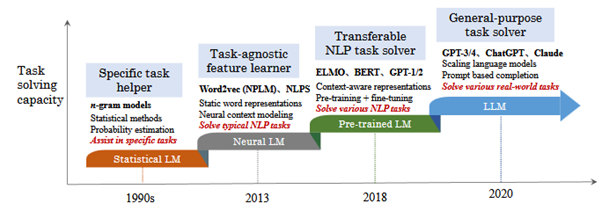
\includegraphics[width=0.85\textwidth]{media/evolusi-llm.png}
\caption[Evolusi LLM berdasarkan kemampuan penyelesaian tugas]{Evolusi LLM berdasarkan kemampuan penyelesaian tugas \citep{zhao_survey_2026}}
\label{fig:evolusi-llm}
\end{figure}

Transformer menggunakan mekanisme perhatian untuk membentuk representasi yang bergantung pada konteks \citep{vaswani_attention_2017}. Model berbasis encoder, seperti BERT, dapat digunakan untuk representasi dan klasifikasi teks; model generatif menghasilkan urutan keluaran berdasarkan masukan dan instruksi \citep{devlin_bert_2019,brown_language_2020}. Dalam pipeline penelitian ini, representasi teks diperlukan untuk pencarian semantik, sedangkan model generatif digunakan untuk ekstraksi, dekomposisi, dan penilaian kandidat. Pilihan model ditentukan oleh kebutuhan tugas dan diuji pada data pengembangan.

Gambar~\ref{fig:arsitektur-transformer} memperlihatkan arsitektur encoder--decoder Transformer, termasuk mekanisme perhatian yang menghubungkan representasi masukan dan keluaran \citep{vaswani_attention_2017}. Gambar ini menjadi landasan untuk membedakan model pembentuk representasi dan model generatif. Penggunaannya dalam penelitian tidak mensyaratkan seluruh model memiliki encoder dan decoder sekaligus; komponen yang digunakan mengikuti arsitektur model embedding atau LLM yang dipilih.

\begin{figure}[!htb]
\centering
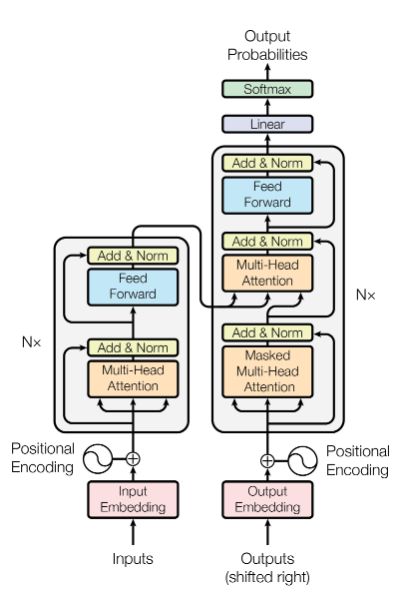
\includegraphics[width=0.75\textwidth,height=0.55\textheight,keepaspectratio]{media/arsitektur-transformer.png}
\caption[Arsitektur Transformer]{Arsitektur Transformer \citep{vaswani_attention_2017}}
\label{fig:arsitektur-transformer}
\end{figure}

\textit{In-context learning} memungkinkan model mengikuti pola tugas melalui instruksi dan contoh tanpa memperbarui parameter model. Pada \textit{few-shot prompting}, sejumlah contoh masukan--keluaran disertakan untuk memperjelas jenis entitas, atribut, serta format hasil yang diharapkan \citep{brown_language_2020}. Contoh perlu dipisahkan dari data uji. Keluaran terstruktur, seperti JSON, memudahkan pemeriksaan kelengkapan atribut dan transformasi ke tahap berikutnya, tetapi validitas format tidak membuktikan kebenaran makna.

Ekstraksi multi-entitas dan dekomposisi kueri mempunyai unit kerja berbeda. Ekstraksi mengubah satu dokumen menjadi sejumlah entitas; dekomposisi mengurai satu entitas atau CDE komposit menjadi konsep utama dan atribut pencarian. Pada CDE-Mapper, dekomposisi mencakup komponen seperti \textit{base entity}, domain, entitas terkait, kategori, satuan, dan kunjungan \citep{gilani_cde-mapper_2025}. Rancangan adaptasi menjalankan dekomposisi terhadap entitas hasil ekstraksi sambil mempertahankan identitas dan konteks sumber.

Misalnya, hasil ekstraksi ``gula darah puasa 126 mg/dL'' dapat diuraikan menjadi konsep pemeriksaan glukosa, konteks puasa, nilai 126, dan satuan mg/dL. Spesimen atau metode yang tidak disebutkan tidak boleh ditambahkan hanya untuk melengkapi struktur. Prinsip ini membatasi informasi yang boleh digunakan untuk membentuk subkueri dan menilai kandidat. Pemeriksaan bukti, validasi struktur, dan penanganan keluaran yang tidak dapat dipastikan diperlukan sebelum hasil diteruskan ke pemetaan.

\section{RAG dan Hybrid Retrieval}

\subsection{Pengambilan Pengetahuan dan Pembentukan Kandidat}

\textit{Retrieval-Augmented Generation} (RAG) menggabungkan pengambilan informasi dari sumber eksternal dengan model generatif \citep{lewis_retrieval-augmented_2021}. Pada pemetaan terminologi, sumber eksternal berupa konsep beserta deskripsi dan metadata, sedangkan keluaran yang diharapkan berupa pemilihan kandidat yang dapat ditelusuri. Secara konseptual, hubungan retriever dan generator dapat diringkas sebagai:
\begin{equation}
 p(y\mid q)=\sum_{z\in Z_k(q)}p_{\eta}(z\mid q)\,p_{\theta}(y\mid q,z),
 \label{eq:rag-probabilistic}
\end{equation}
 dengan $q$ sebagai kueri, $Z_k(q)$ sebagai konteks terambil, $p_{\eta}$ sebagai distribusi retriever, dan $p_{\theta}$ sebagai distribusi keluaran generator. Persamaan ini menjelaskan ketergantungan hasil pada konteks dan model; implementasi pemeringkatan kandidat tidak harus menghitung marginalisasi tersebut secara eksplisit.

Gambar~\ref{fig:arsitektur-rag} menunjukkan hubungan masukan, retriever, penggabungan konteks, dan generator dalam arsitektur umum RAG \citep{wu_retrieval-augmented_2025}. Dalam pemetaan terminologi, konteks eksternal berupa kandidat konsep beserta metadata, sedangkan generator digunakan untuk menilai kesesuaiannya terhadap kueri dan konteks klinis. Dengan demikian, kualitas pemetaan bergantung pada keberhasilan mengambil kandidat sekaligus kemampuan model menggunakan bukti tersebut.

\begin{figure}[!htb]
\centering
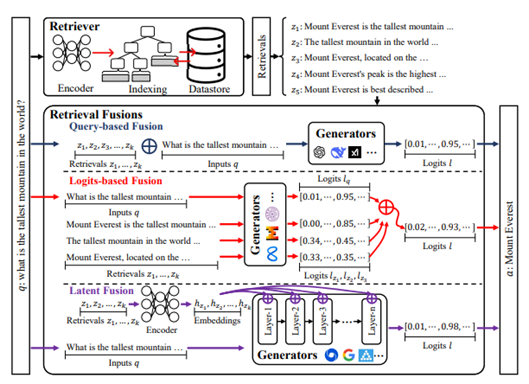
\includegraphics[width=0.9\textwidth]{media/arsitektur-rag.png}
\caption[Arsitektur umum RAG]{Arsitektur umum RAG \citep{wu_retrieval-augmented_2025}}
\label{fig:arsitektur-rag}
\end{figure}


Perbedaan Naive RAG, Advanced RAG, dan Modular RAG pada Gambar~\ref{fig:evolusi-rag} memperlihatkan perluasan alur dasar pengambilan dan pembangkitan dengan optimasi kueri, pemrosesan kandidat, serta modul yang dapat disesuaikan \citep{gao_retrieval-augmented_2024}. Bagi penelitian ini, gambaran tersebut menjelaskan penempatan normalisasi dan dekomposisi sebelum pencarian, serta filtering dan reranking setelah pencarian. Ketiga paradigma merupakan konteks konseptual; konfigurasi yang diuji tetap mengikuti rancangan eksperimen Bab IV.

\begin{figure}[!htb]
\centering
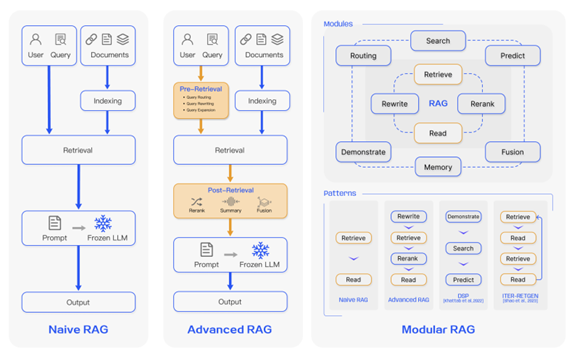
\includegraphics[width=0.9\textwidth]{media/evolusi-rag.png}
\caption[Paradigma dalam evolusi RAG]{Paradigma dalam evolusi RAG \citep{gao_retrieval-augmented_2024}}
\label{fig:evolusi-rag}
\end{figure}


CDE-Mapper mengoperasionalkan pemetaan melalui dekomposisi, retrieval, filtering, reranking, dan reservoir seperti pada Gambar~\ref{fig:framework-cde-mapper} \citep{gilani_cde-mapper_2025}. Gambar ini menunjukkan fondasi baseline; lapisan normalisasi dan ekstraksi multi-entitas Bahasa Indonesia dijelaskan dalam arsitektur adaptasi pada Bab IV.

\begin{figure}[!htb]
\centering
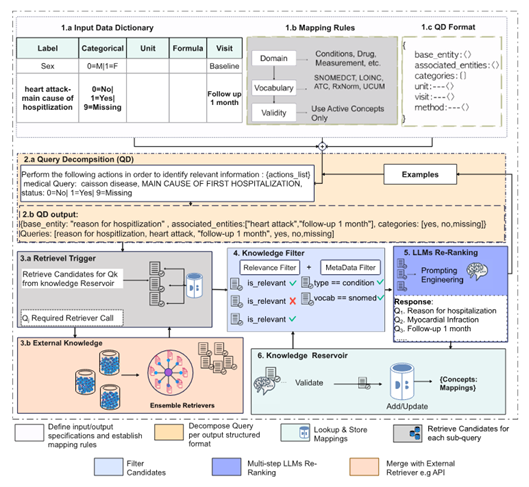
\includegraphics[width=0.9\textwidth]{media/framework-cde-mapper.png}
\caption[Framework CDE-Mapper]{Framework CDE-Mapper \citep{gilani_cde-mapper_2025}}
\label{fig:framework-cde-mapper}
\end{figure}

\subsection{Sparse, Dense, dan Penggabungan Hasil}

\textit{Dense retrieval} merepresentasikan kueri dan kandidat sebagai vektor padat. SapBERT memanfaatkan penyelarasan sinonim biomedis untuk membentuk representasi nama entitas \citep{liu_self-alignment_2021}. Kemiripan dapat dihitung dengan cosine similarity:
\begin{equation}
 s_{\mathrm{dense}}(q,c)=\frac{\mathbf{e}_{q}^{\top}\mathbf{e}_{c}}{\lVert\mathbf{e}_{q}\rVert_2\lVert\mathbf{e}_{c}\rVert_2},
 \label{eq:dense-retrieval}
\end{equation}
 dengan $\mathbf{e}_{q}$ dan $\mathbf{e}_{c}$ sebagai vektor kueri dan kandidat yang tidak bernilai nol. Kemampuan menyelaraskan sinonim biomedis tidak otomatis membuktikan kemampuan lintas bahasa untuk seluruh istilah Indonesia; kesesuaian representasinya tetap menjadi objek evaluasi.

\textit{Sparse retrieval} menggunakan representasi berbobot pada ruang kosakata $V$. SPLADE mempelajari bobot dan ekspansi leksikal dalam representasi jarang \citep{formal_splade_2021}. Skor pencocokan dinyatakan sebagai:
\begin{equation}
 s_{\mathrm{sparse}}(q,c)=\mathbf{w}_{q}^{\top}\mathbf{w}_{c}=\sum_{t\in V}w_{q,t}w_{c,t}.
 \label{eq:sparse-retrieval}
\end{equation}
 Kedua jalur menyediakan bukti yang saling melengkapi. Setelah skor disetarakan skalanya, salah satu bentuk penggabungan adalah:
\begin{equation}
 s_{\mathrm{hybrid}}(q,c)=\alpha\widetilde{s}_{\mathrm{sparse}}(q,c)+(1-\alpha)\widetilde{s}_{\mathrm{dense}}(q,c),\quad 0\leq\alpha\leq1,
 \label{eq:hybrid-retrieval}
\end{equation}
 dengan tanda tilde menyatakan skor ternormalisasi dan $\alpha$ mengatur bobot leksikal. Kandidat kemudian dipilih dari basis pengetahuan $\mathcal{K}$:
\begin{equation}
 C_k(q)=\operatorname{TopK}_{c\in\mathcal{K}}s_{\mathrm{hybrid}}(q,c).
 \label{eq:topk-candidate-set}
\end{equation}
 Penggabungan berbobot tersebut merupakan pilihan metode penelitian, bukan pernyataan tentang algoritma fusi asli CDE-Mapper. Model sparse, prosedur normalisasi skor, bobot, serta nilai $k$ harus ditetapkan dan dilaporkan dalam eksperimen.

\subsection{Routing dan Filtering}

Routing memilih ruang pencarian berdasarkan jenis entitas dan tujuan representasinya. Filtering menyaring kandidat berdasarkan metadata atau bukti kesesuaian setelah kandidat tersedia. Keduanya dapat menggunakan domain, terminologi target, status konsep, serta atribut klinis, tetapi bekerja pada titik berbeda dalam pipeline \citep{gilani_cde-mapper_2025}. Pembatasan yang terlalu ketat dapat menghilangkan kandidat benar, sedangkan pembatasan yang terlalu longgar menambah kandidat tidak relevan.

Dalam penelitian ini, diagnosis dapat memerlukan representasi klinis dan klasifikasi, sementara pemeriksaan memerlukan identifikasi observasi. Ruang pencarian karena itu dapat mencakup lebih dari satu terminologi sesuai kebutuhan. Aturan domain tidak menggantikan pemeriksaan konteks, dan skor kemiripan tidak diperlakukan sebagai probabilitas kebenaran yang telah terkalibrasi. Dampak routing dan filtering diuji melalui ablasi sebagaimana dirancang pada Bab IV.

\section{Reranking, Validasi, dan Knowledge Reservoir}

Reranking menilai ulang kandidat dengan informasi yang lebih lengkap daripada skor retrieval awal. Penilaian dapat mempertimbangkan label, sinonim, domain, atribut, serta tingkat kekhususan konsep. CDE-Mapper menggunakan penilaian relevansi dan klasifikasi hubungan kandidat, termasuk kategori exact, highly relevant, partially relevant, dan not relevant \citep{gilani_cde-mapper_2025}. Kandidat yang dekat secara semantik tetap dapat tidak tepat apabila menambahkan rincian yang tidak didukung sumber.

\textit{Self-consistency} mengagregasi beberapa keluaran untuk memperoleh keputusan yang lebih stabil \citep{wang_self-consistency_2023}. Konsistensi perlu dibedakan dari ketepatan: model dapat berulang kali menghasilkan keputusan salah. Karena itu, keputusan penerimaan dalam rancangan penelitian tetap mempertimbangkan label relevansi, konflik atribut, dan ambang penerimaan. Abstain digunakan ketika bukti belum memadai sehingga kasus memerlukan peninjauan ahli. Formula skor gabungan dan aturan penerimaan merupakan operasionalisasi model usulan pada Bab IV.

\textit{Knowledge reservoir} menyimpan pemetaan agar kasus berulang dapat menggunakan kembali hasil sebelumnya \citep{gilani_cde-mapper_2025}. Penggunaan ulang perlu memperhatikan konteks, domain, serta versi terminologi; label teks yang sama belum tentu mewakili kasus setara. Pada rancangan penelitian ini, penyimpanan pemetaan tervalidasi ahli dibedakan dari keluaran yang baru dinilai otomatis oleh LLM. Reservoir juga dibedakan dari indeks konsep untuk retrieval dan dari gold standard evaluasi.

Dengan demikian, validasi mencakup pemeriksaan format, kesesuaian terhadap bukti sumber, dan ketepatan konsep. Evaluasi reservoir memerlukan kondisi cold cache dan warm cache yang dinyatakan jelas. Data uji tidak digunakan untuk mengisi jawaban reservoir sebelum pengujian. Prinsip ini menjaga keterlacakan keputusan sekaligus memungkinkan penilaian manfaat komputasinya.

\section{Prinsip Evaluasi}

Evaluasi memisahkan ekstraksi, retrieval, dan keputusan pemetaan agar sumber kesalahan dapat diketahui. Unit evaluasi ditetapkan sebelum eksperimen: span bertipe untuk ekstraksi, pasangan entitas--terminologi untuk mapping, dan dokumen untuk evaluasi end-to-end. Gold standard, penyelesaian perbedaan anotasi, serta pembagian data dijelaskan pada Bab IV. Tabel~\ref{tab:ringkasan-metrik-evaluasi} merangkum fungsi metrik.

\begin{table}[htbp]
\centering
\small
\caption{Metrik evaluasi menurut tahap pipeline}
\label{tab:ringkasan-metrik-evaluasi}
\begin{tabularx}{\textwidth}{@{}>{\raggedright\arraybackslash}p{2.5cm} >{\raggedright\arraybackslash}X >{\raggedright\arraybackslash}X@{}}
\toprule
\textbf{Tahap} & \textbf{Metrik} & \textbf{Fokus penilaian} \\
\midrule
Ekstraksi & Precision, recall, F1; accuracy atau macro-F1 atribut. & Ketepatan span, tipe, dan konteks. \\
Retrieval & Recall@k, Top-k accuracy, MRR. & Kehadiran dan posisi kandidat benar. \\
Mapping & Accuracy@1; precision, recall, F1 end-to-end. & Ketepatan kode dan hasil pipeline. \\
Validasi & Coverage, konsistensi, agreement anotator. & Cakupan, kestabilan, dan mutu anotasi. \\
Efisiensi & Latensi, token, cache hit. & Beban komputasi dan penggunaan ulang. \\
\bottomrule
\end{tabularx}
\end{table}

\subsection{Ketepatan Ekstraksi dan Pemetaan}

Untuk $N$ kasus pemetaan yang memiliki padanan gold, akurasi kandidat utama didefinisikan sebagai:
\begin{equation}
 \mathrm{Accuracy@1}=\frac{1}{N}\sum_{i=1}^{N}\mathbf{1}(\widehat{c}_i\in G_i),
 \label{eq:accuracy}
\end{equation}
 dengan $G_i$ sebagai himpunan padanan yang diterima untuk kasus ke-$i$ dan $\widehat{c}_i$ sebagai hasil sistem. Abstain pada kasus yang memiliki padanan gold dihitung sebagai tidak benar pada ukuran ini. Akurasi bersyarat pada hasil yang diterima dilaporkan terpisah, sedangkan kasus tanpa padanan gold memerlukan evaluasi keputusan abstain tersendiri.

Pada ekstraksi, TP adalah prediksi yang cocok dengan span dan tipe gold, FP adalah prediksi yang tidak cocok, dan FN adalah entitas gold yang tidak ditemukan. Pada evaluasi end-to-end, kecocokan juga mensyaratkan kode dan terminologi target yang benar. Pencocokan dilakukan satu-ke-satu agar duplikasi prediksi tidak menambah TP.
\begin{align}
 \mathrm{Precision}&=\frac{TP}{TP+FP},\label{eq:precision}\\
 \mathrm{Recall}&=\frac{TP}{TP+FN},\label{eq:recall}\\
 F1&=\frac{2\,\mathrm{Precision}\,\mathrm{Recall}}{\mathrm{Precision}+\mathrm{Recall}}.\label{eq:f1score}
\end{align}
 Aturan kecocokan strict atau relaxed, agregasi micro atau macro, serta penanganan penyebut nol harus dinyatakan dalam protokol evaluasi. Evaluasi atribut konteks dilaporkan dengan menyebutkan apakah menggunakan entitas gold atau hanya entitas yang berhasil dicocokkan.

\subsection{Kualitas Kandidat dan Cakupan}

Jika $C_i^{(k)}$ adalah daftar Top-$k$ dan $R_i$ adalah himpunan konsep relevan, ukuran retrieval dirumuskan sebagai:
\begin{align}
 \mathrm{Top\text{-}}k\ \mathrm{Accuracy}&=\frac{1}{N}\sum_{i=1}^{N}\mathbf{1}\!\left(R_i\cap C_i^{(k)}\neq\varnothing\right),\label{eq:topk}\\
 \mathrm{Recall@}k&=\frac{1}{N}\sum_{i=1}^{N}\frac{|R_i\cap C_i^{(k)}|}{|R_i|},\label{eq:recallatk}\\
 \mathrm{MRR}&=\frac{1}{N}\sum_{i=1}^{N}\mathrm{RR}_i,\quad
 \mathrm{RR}_i=\begin{cases}1/r_i,&\text{kandidat relevan ditemukan},\\0,&\text{selainnya}.\end{cases}\label{eq:mrr}
\end{align}
 Di sini $r_i$ adalah peringkat kandidat relevan pertama. Recall@k dihitung pada kasus dengan $|R_i|>0$. Untuk satu konsep relevan per kueri, Recall@k sama dengan Top-k accuracy; untuk beberapa konsep, keduanya mengukur hal berbeda. Batas kedalaman daftar pada penghitungan MRR perlu dilaporkan.

Coverage kandidat menunjukkan proporsi masukan yang memperoleh setidaknya satu kandidat valid setelah filtering:
\begin{equation}
 \mathrm{Coverage}_{\mathrm{kandidat}}=\frac{N_{\mathrm{masukan\ dengan\ kandidat\ valid}}}{N_{\mathrm{seluruh\ masukan}}}.
 \label{eq:coverage}
\end{equation}
 Valid di sini berarti memenuhi batasan ruang pencarian, bukan telah terbukti benar menurut gold. Coverage keputusan akhir dihitung sebagai proporsi kasus yang diterima tanpa abstain dan dilaporkan terpisah. Pemisahan ini mencegah daftar kandidat yang selalu terisi dianggap sebagai keberhasilan pemetaan.

\subsection{Konsistensi, Agreement, dan Efisiensi}

Untuk $T\geq2$ pengulangan pada masukan yang sama, salah satu ukuran konsistensi adalah proporsi pasangan keputusan yang sama:
\begin{equation}
 \mathrm{Consistency}=\frac{\sum_{t<u}\mathbf{1}(L^{(t)}=L^{(u)})}{\binom{T}{2}}.
 \label{eq:consistency}
\end{equation}
 Ukuran ini dirata-ratakan pada kasus yang diuji. Ia berbeda dari proporsi suara mayoritas yang digunakan sebagai komponen skor kandidat pada Bab IV; keduanya harus dilaporkan sesuai definisinya. Konsistensi tidak menggantikan pembandingan dengan gold standard.

Kesepakatan anotator untuk keputusan kategorikal dapat dinilai dengan koefisien Kappa:
\begin{equation}
 \kappa=\frac{P_o-P_e}{1-P_e},
 \label{eq:kappa}
\end{equation}
 dengan $P_o$ sebagai kesepakatan teramati dan $P_e$ sebagai kesepakatan yang diharapkan secara kebetulan. Varian Kappa dipilih sesuai jumlah anotator dan desain penilaian. Untuk anotasi span bebas, kecocokan span dan tipe perlu diperiksa terlebih dahulu; agreement atribut dihitung pada unit yang dapat dibandingkan. Agreement anotator dan konsistensi LLM merupakan dua objek evaluasi berbeda.

Efisiensi diukur dengan waktu inferensi per unit masukan:
\begin{equation}
 \bar{t}_{\mathrm{inferensi}}=\frac{1}{N}\sum_{i=1}^{N}t_i,
 \label{eq:efficiency-time}
\end{equation}
 serta persentase pengurangan waktu terhadap baseline:
\begin{equation}
 \mathrm{Pengurangan\ waktu}(\%)=\frac{t_{\mathrm{baseline}}-t_{\mathrm{usulan}}}{t_{\mathrm{baseline}}}\times100\%.
 \label{eq:speedup}
\end{equation}

% Hindari satu baris penutup terpisah pada halaman baru.
\enlargethispage{\baselineskip}
 Nilai positif menunjukkan waktu lebih singkat; ukuran ini berbeda dari rasio speedup $t_{\mathrm{baseline}}/t_{\mathrm{usulan}}$. Perbandingan menggunakan beban kerja dan lingkungan yang sebanding, disertai jumlah panggilan LLM, penggunaan token, dan kondisi cache. Landasan evaluasi ini mendukung pengujian tiga rumusan masalah melalui pemetaan per terminologi, ekstraksi teks panjang, dan adaptasi Bahasa Indonesia pada Bab IV.




% Bab IV
\chapter{METODE PENELITIAN}

\section{Gambaran Umum Penelitian}

Penelitian ini bertujuan untuk mengembangkan dan mengevaluasi sebuah \textit{framework} adaptif untuk pemetaan terminologi klinis Bahasa Indonesia ke kosakata terkendali standar, seperti SNOMED CT, LOINC, dan ICD-10. Pendekatan utama yang diusulkan adalah adaptasi dari arsitektur CDE-Mapper \citep{gilani_cde-mapper_2025} dengan optimalisasi komponen ekstraksi teks klinis yang menggunakan bahasa Indonesia dan berupa teks panjang.

\section{Tahapan Penelitian}

Penelitian ini akan dilaksanakan dalam lima tahapan utama seperti digambarkan pada Gambar~\ref{fig:tahapan-penelitian}.


\begin{figure}[H]
    \centering
    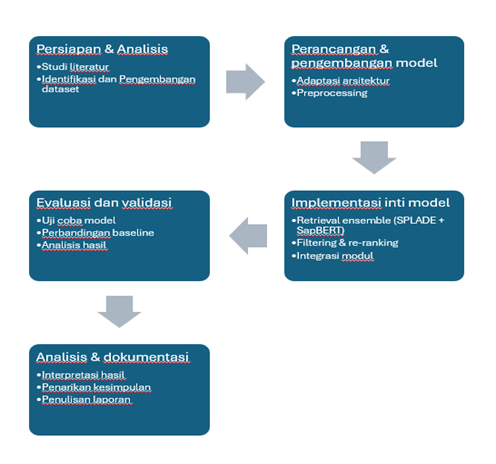
\includegraphics[width=0.8\textwidth]{media/tahapan_penelitian.png}
    \caption{Tahapan penelitian}
    \label{fig:tahapan-penelitian}
\end{figure}

Penelitian ini dilaksanakan dalam lima tahapan utama yang saling terkait secara berurutan maupun iteratif. Kelima tahapan pada Gambar~\ref{fig:tahapan-penelitian} dijelaskan sebagai berikut.

\subsection{Persiapan dan Analisis}

Tahap ini bertujuan untuk membangun fondasi teoritis dan menyiapkan sumber daya data yang diperlukan sebelum memasuki pengembangan model.

\subsubsection{Studi Literatur}

Studi literatur dilakukan secara sistematis untuk mengidentifikasi \textit{state-of-the-art} dalam pemetaan terminologi klinis. Ruang lingkup literatur mencakup standar interoperabilitas kesehatan, seperti FHIR, SNOMED CT, LOINC, dan ICD-10, serta implementasinya di SATUSEHAT \citep{ayuningtyas_bringing_2025,heryawan_fast_2025}; metode pemetaan dari \textit{rule-based}, \textit{machine learning}, \textit{deep learning}, hingga LLM dan RAG \citep{meizoso_automated_2011,hristov_application_2021,gilani_cde-mapper_2025}; serta arsitektur CDE-Mapper dan keterbatasannya dalam memproses teks panjang dengan \textit{multiple CDE} komposit \citep{gilani_cde-mapper_2025}. Hasil studi literatur digunakan untuk merumuskan kerangka konseptual dan menentukan komponen kunci yang akan diadaptasi.

\subsubsection{Identifikasi dan Pengembangan Dataset}

Kegiatan ini mencakup identifikasi sumber data istilah klinis Bahasa Indonesia. Data diperoleh dari rekam medis elektronik (RME) puskesmas atau klinik swasta, dan platform konsultasi kesehatan daring yang telah dianonimkan. Sumber-sumber ini dipilih karena merepresentasikan variasi nyata istilah lokal, singkatan, dan kesalahan eja \citep{purwitasari_comparison_2023,hossain_exploratory_2025}. Selain itu, dikumpulkan pula kosakata terkendali standar berupa SNOMED CT, LOINC, dan ICD-10 sebagai terminologi target.

Pembangunan dataset emas (\textit{gold standard}) dilakukan dengan menganotasi sampel 100--200 istilah klinis secara manual oleh tenaga medis, seperti dokter atau perekam medis, dengan kode standar yang sesuai. Validasi antar-anotator (\textit{inter-annotator agreement}) dihitung menggunakan koefisien Kappa Fleiss untuk menjamin konsistensi. Dataset emas ini menjadi kebenaran dasar untuk evaluasi performa model.

\subsection{Perancangan dan Pengembangan Model}

Pada tahap ini, arsitektur model usulan dirancang dan komponen \textit{preprocessing} dikembangkan secara spesifik untuk teks klinis panjang dalam bahasa Indonesia.

\subsubsection{Adaptasi Arsitektur}

Arsitektur CDE-Mapper diadaptasi dengan penambahan modul dekomposisi teks panjang dalam bahasa Indonesia. Karena CDE-Mapper asli hanya menerima satu CDE per \textit{input}, ditambahkan modul yang memecah dokumen klinis panjang menjadi unit-unit kalimat atau klausa yang mengandung CDE potensial. Pendekatan ini menggunakan aturan pemisah kalimat, dan deteksi frasa klinis berbasis pola.

Optimasi \textit{LLM-based query decomposition} untuk \textit{retrieval ensemble} dilakukan agar sesuai dengan karakteristik istilah klinis Bahasa Indonesia dan kebutuhan \textit{multi-terminology mapping}. Selain itu, diintegrasikan pula mekanisme \textit{confidence-based selection} yang diadaptasi dari pendekatan hibrida normalisasi konsep klinis oleh \citet{chen_clinical_2020} untuk menangani ketidakpastian dan merekomendasikan kandidat yang perlu validasi manual.

\subsubsection{Preprocessing}

\textit{Preprocessing} dirancang khusus untuk membersihkan dan menstandarkan teks klinis sebelum masuk ke pemrosesan lanjutan. Langkah-langkahnya meliputi \textit{case folding} (semua teks diubah menjadi huruf kecil); normalisasi singkatan medis menggunakan kamus singkatan yang dibangun dari literatur dan buku rekam medis, misalnya DM'' menjadidiabetes mellitus'' dan TD'' menjaditekanan darah''; \textit{stemming} Bahasa Indonesia untuk mengurangi kata berimbuhan ke bentuk dasar secara selektif; penanganan variasi ejaan dan istilah sehari-hari; serta segmentasi kalimat untuk menjaga konteks lokal setiap entitas. Tahap ini hanya bertujuan menyiapkan teks bersih dan tidak melakukan pemetaan konsep.

\subsection{Implementasi Inti Model}

Implementasi inti model dibangun dalam sebuah \textit{pipeline} berbasis Python yang mengintegrasikan enam komponen utama secara berurutan. Pertama, ekstraksi multi-entitas dari teks klinis menjadi objek JSON terstruktur, yang memuat entitas utama, domain, kategori, unit, metode, negasi, dan konteks temporal. Kedua, penerapan aturan pemetaan berbasis domain untuk menentukan terminologi target (SNOMED CT, LOINC, atau ICD-10), dilanjutkan dengan dekomposisi kueri menjadi komponen atomik guna menghindari ambiguitas pencarian. Ketiga, pemeriksaan \textit{knowledge reservoir} untuk mengambil hasil tervalidasi jika tersedia dan menghindari komputasi ulang. Keempat, \textit{retrieval ensemble} yang memanfaatkan SPLADE untuk pencarian leksikal dan SapBERT untuk pencarian semantik, guna menghasilkan daftar kandidat konsep standar dari basis pengetahuan terminologi. Kelima, \textit{filtering} dan \textit{re-ranking} untuk menyaring kandidat yang tidak sesuai domain, atribut, atau status aktif, serta menilai ulang kesesuaiannya terhadap konteks kalimat secara keseluruhan. Keenam, validasi keputusan melalui agregasi penilaian, dengan keluaran akhir berupa kandidat final beserta skor kepercayaan, atau status \textit{abstain} yang memerlukan validasi ahli jika tidak ada kandidat yang memenuhi ambang penerimaan.

\subsection{Evaluasi dan Validasi}

Tahap ini menguji performa model secara kuantitatif dan kualitatif.

\subsubsection{Uji Coba Model}

Model diuji pada dataset emas dengan skenario sebagai berikut.

\begin{enumerate}
    \item Uji standar: menggunakan istilah yang sudah baku dalam dataset.
    \item Uji variasi leksikal: menggunakan istilah dengan singkatan, ejaan salah, atau bahasa sehari-hari yang diambil dari platform konsultasi daring \citep{purwitasari_comparison_2023}.
    \item Uji teks panjang: menggunakan dokumen klinis naratif, misalnya catatan perkembangan pasien, yang mengandung beberapa CDE komposit. Model harus mengekstraksi seluruh CDE dan memetakannya.
    \item Uji ablasi: model dijalankan tanpa komponen tertentu, yaitu tanpa modul \textit{rule-based}, tanpa SapBERT, dan tanpa \textit{cross-encoder}, untuk mengukur kontribusi masing-masing komponen.
    \item Perbandingan \textit{baseline}: perbandingan utama yang akan dilakukan adalah membandingkan \textit{framework} usulan dengan CDE-Mapper original \citep{gilani_cde-mapper_2025}. Jika memungkinkan, simulasi dengan LLM kecil akan digunakan untuk proses dekomposisi dengan anggaran komputasi yang dibatasi.
\end{enumerate}

\subsubsection{Analisis Hasil}

Hasil kuantitatif disajikan dalam tabel dan grafik perbandingan. Analisis statistik, misalnya uji-\textit{t} berpasangan, dilakukan untuk menentukan signifikansi perbedaan antar model. Selain itu, dilakukan analisis kesalahan (\textit{error analysis}) dengan mengelompokkan kesalahan pemetaan ke dalam kategori berikut.

\begin{enumerate}
    \item Kesalahan karena variasi leksikal, misalnya singkatan yang tidak dikenal.
    \item Kesalahan karena ambiguitas semantik, yaitu satu istilah dapat merujuk ke dua konsep berbeda.
    \item Kesalahan karena kegagalan ekstraksi CDE dari teks panjang.
    \item Kesalahan karena keterbatasan pengetahuan terminologi, yaitu ketika konsep tidak ada di basis data.
\end{enumerate}

Setiap kesalahan dianalisis secara kualitatif untuk memberikan rekomendasi perbaikan.

\subsection{Analisis dan Dokumentasi}

Tahap akhir penelitian ini berfokus pada interpretasi, penarikan kesimpulan, dan penulisan laporan.

\subsubsection{Interpretasi Hasil}

Hasil evaluasi diinterpretasikan dalam kerangka pertanyaan penelitian: seberapa baik \textit{framework} usulan memetakan terminologi klinis Bahasa Indonesia dibandingkan \textit{baseline}; bagaimana kontribusi masing-masing komponen, seperti dekomposisi, \textit{retrieval ensemble}, dan \textit{preprocessing}, terhadap peningkatan akurasi; apakah model mampu menangani teks panjang dengan \textit{multiple CDE} komposit secara simultan; dan seberapa efisien model digunakan untuk teks klinis dalam bahasa Indonesia.

\subsubsection{Penarikan Kesimpulan}

Kesimpulan dirumuskan berdasarkan tujuan penelitian yang ditetapkan di Bab I. \textit{Framework} adaptif yang dikembangkan diharapkan mampu mengatasi keterbatasan CDE-Mapper asli dalam memproses teks klinis panjang dan mengenali \textit{multiple CDE}. Pendekatan \textit{hybrid rule-based} dan \textit{semantic retrieval} diharapkan efektif untuk konteks \textit{low-resource} bahasa Indonesia dengan akurasi yang kompetitif. Rekomendasi juga diberikan untuk implementasi di SATUSEHAT dan penelitian lanjutan, termasuk perlunya validasi klinis yang lebih luas dan pengembangan mekanisme \textit{active learning} untuk memperbaiki model secara berkelanjutan.

\subsubsection{Penulisan Laporan}

Seluruh proses, desain, implementasi, data, hasil, dan kesimpulan didokumentasikan secara sistematis dalam naskah disertasi sesuai panduan penulisan Universitas Gadjah Mada. Laporan juga mencakup kode sumber pada repositori pendukung dan dataset anonim yang digunakan sehingga penelitian ini dapat direproduksi dan dikembangkan lebih lanjut oleh peneliti lain.

\section{Deskripsi Usulan Model}

Arsitektur model yang diusulkan untuk mengadaptasi CDE-Mapper agar mampu melakukan pemetaan terminologi klinis secara \textit{end-to-end} dari teks klinis panjang berbahasa Indonesia, menjadi kode standar, yaitu SNOMED CT, LOINC, dan ICD-10. Model diusulkan sebagai \textit{pipeline hybrid} yang menggabungkan ekstraksi entitas berbasis LLM, \textit{retrieval} semantik dan leksikal (\textit{dense} + \textit{sparse}), serta mekanisme validasi dan penyimpanan pengetahuan (\textit{knowledge reservoir}) untuk meningkatkan akurasi dan efisiensi inferensi \citep{gilani_cde-mapper_2025}.

\subsection{Tujuan dan Keluaran Model}

Secara operasional, model menerima masukan berupa: (1) teks klinis panjang berbahasa Indonesia, misalnya resume medis, catatan perkembangan, atau hasil penunjang; atau (2) daftar istilah atau \textit{field} dari kamus data RME. Keluaran yang diharapkan adalah daftar \textit{clinical data elements} (CDE) hasil ekstraksi beserta pasangan pemetaan ke terminologi target, yang mencakup \textit{mention} asli, tipe entitas, normalisasi istilah, kandidat kode teratas (Top-\textit{k}), skor kepercayaan, serta keputusan akhir, yaitu \textit{exact}, \textit{highly}, \textit{partial}, atau \textit{not relevant}. Untuk kasus komposit, keluaran juga menyertakan dekomposisi atribut, yaitu \textit{Base entity}, \textit{Domain}, \textit{Additional Entities}, \textit{categories}, \textit{Unit}, \textit{Visit}, dan \textit{Method} \citep{gilani_cde-mapper_2025}.


\subsection{Arsitektur, Alur Proses, dan Komponen Utama}

Arsitektur usulan mengadopsi komponen utama CDE-Mapper \citep{gilani_cde-mapper_2025}, kemudian menambahkan lapisan NLP untuk mengubah teks klinis naratif berbahasa Indonesia menjadi sekumpulan CDE terstruktur. Adaptasi ini berfokus pada: (i) penanganan variasi bahasa klinis Indonesia, seperti singkatan, istilah lokal, ejaan tidak baku, negasi, dan konteks temporal; (ii) pemrosesan teks panjang yang dapat mengandung banyak entitas, bukan hanya satu CDE pada setiap masukan; dan (iii) pemetaan ke tiga terminologi dalam ruang lingkup penelitian, yaitu SNOMED CT, LOINC, dan ICD-10.

Secara operasional, arsitektur merupakan rangkaian delapan langkah: pra-pemrosesan dan normalisasi bahasa; ekstraksi multi-entitas dan pembentukan JSON; penerapan \textit{mapping rules} serta transformasi format; dekomposisi kueri secara \textit{batch}; pemeriksaan \textit{knowledge reservoir}; \textit{ensemble retrieval}; \textit{filtering}, \textit{reranking}, dan validasi; serta pembaruan \textit{knowledge reservoir}. Rangkaian tersebut menghubungkan modul NLP yang menjadi kontribusi adaptasi dengan algoritma CDE-Mapper.

\begin{figure}[H]
    \centering
    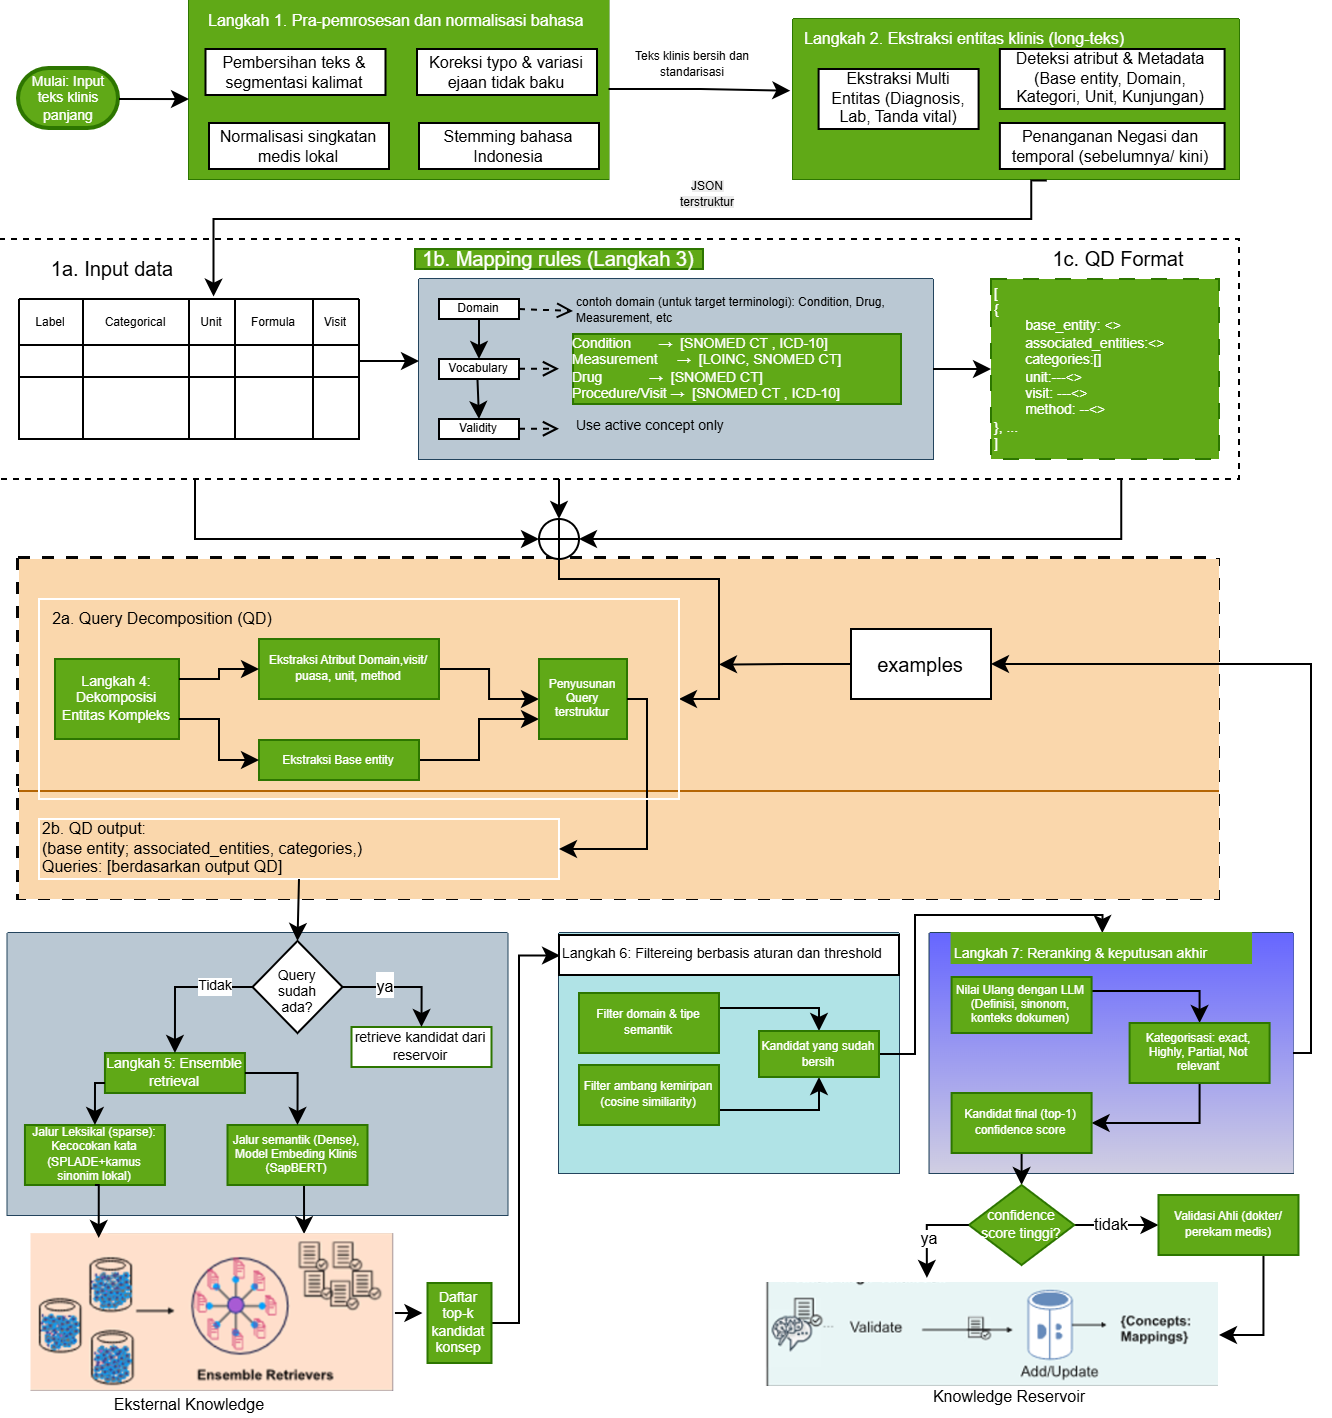
\includegraphics[width=0.95\textwidth]{media/Framework Usulan 25062026-Rev2 Agst.png}
    \caption{Framework adaptasi pemetaan terminologi klinis Bahasa Indonesia}
    \label{fig:alur-operasional-mapping}
\end{figure}

Bagian berarsir hijau pada Gambar~\ref{fig:alur-operasional-mapping} menunjukkan komponen yang ditambahkan atau disesuaikan untuk Bahasa Indonesia. Penjelasan setiap langkah adalah sebagai berikut.

\Needspace{6\baselineskip}
\begin{enumerate}
    \item \textbf{Pra-pemrosesan dan normalisasi bahasa.}
    \begin{itemize}
        \item \textbf{Fungsi:} membersihkan teks, melakukan segmentasi kalimat, memperbaiki ejaan tidak baku, menormalkan singkatan medis, melakukan \textit{stemming}, serta menstandarkan simbol, angka, dan satuan tanpa menghilangkan informasi klinis penting.
        \item \textbf{Pembersihan teks:} karakter berulang, emotikon, spasi berlebih, dan pemisah baris yang tidak informatif dibersihkan. Implementasi awal dapat memanfaatkan dan menyesuaikan modul \textit{text-normalization} untuk karakteristik data klinis \citep{utomo_text_normalization}.
        \item \textbf{Segmentasi kalimat:} dokumen panjang dibagi menjadi kalimat atau segmen koheren agar konteks lokal setiap entitas tetap terjaga. Model segmentasi berbasis transformer untuk Bahasa Indonesia dapat digunakan sebagai acuan atau pembanding \citep{Hananto2026}.
        \item \textbf{Koreksi bentuk tidak baku:} variasi informal, salah eja, dan pengulangan huruf dinormalkan menggunakan kamus dan aturan yang dapat diadaptasi dari \textit{indo-normalizer} \citep{dyasputro_indo_normalizer}.
        \item \textbf{Normalisasi singkatan medis:} singkatan seperti ``Px'', ``dgn'', ``DM'', ``GDP'', dan ``TD'' diperluas menggunakan kamus singkatan medis lokal. Kamus awal mengacu pada daftar singkatan rekam medis dan selanjutnya divalidasi oleh ahli \citep{RSI_Sultan_Agung_2019}.
        \item \textbf{Stemming selektif:} kata berimbuhan dapat dikembalikan ke bentuk dasar menggunakan Sastrawi \citep{librian_sastrawi}. Stemming tidak diterapkan pada kode, nama obat, nilai numerik, dan istilah yang berisiko berubah makna klinis.
        \item \textbf{Contoh input:} ``Px dgn DM tipe 2, GDP 126 mg/dL, TD 150/90''.
        \item \textbf{Contoh keluaran:} ``pasien dengan diabetes mellitus tipe 2, gula darah puasa 126 mg/dL, tekanan darah 150/90''.
        \item \textbf{Keluaran tahap:} teks klinis bersih yang siap diproses oleh modul ekstraksi entitas.
    \end{itemize}

    \Needspace{6\baselineskip}
    \item \textbf{Ekstraksi multi-entitas dan pembentukan JSON.}
    \begin{itemize}
        \item \textbf{Fungsi:} mendeteksi banyak entitas klinis dari setiap segmen menggunakan LLM atau model NER medis. Model medis yang menyediakan keluaran NER terstruktur, seperti Numind Medical NER LLM, dapat digunakan sebagai salah satu kandidat dan dibandingkan dengan LLM melalui pendekatan \textit{few-shot} \citep{johnsnowlabs2026numind}.
        \item \textbf{Informasi yang dideteksi:} entitas utama, domain, kategori atau nilai kategorikal, unit, metode atau formula, kunjungan, atribut tambahan, status negasi, dan konteks temporal. Instruksi atau aturan khusus digunakan agar frasa seperti ``tidak ada'', ``bukan'', dan ``tanpa'' ditandai sebagai negasi, sedangkan ``sebelumnya'', ``dulu'', ``kini'', dan ``saat ini'' diberi penanda waktu.
        \item \textbf{Output terstruktur:} setiap entitas disimpan sebagai objek JSON. \textit{Label} memuat nama CDE atau frasa klinis utama; \textit{categorical} memuat daftar atau pasangan kategori nilai; \textit{unit} memuat satuan pengukuran; \textit{formula} memuat aturan perhitungan atau hubungan antarelemen apabila CDE merupakan hasil turunan; dan \textit{visit} memuat konteks kunjungan atau waktu pengukuran. Metadata tambahan seperti \textit{domain}, \textit{method}, \textit{assertion}, dan \textit{temporal} dipertahankan untuk membantu pemetaan.
        \item \textbf{Contoh hasil:} ``diabetes mellitus tipe 2'' sebagai diagnosis; ``gula darah puasa 126 mg/dL'' sebagai pemeriksaan laboratorium; dan ``tekanan darah 150/90'' sebagai tanda vital.
        \item \textbf{Keluaran tahap:} daftar \textit{mention} terstruktur sehingga satu dokumen panjang dapat menghasilkan beberapa CDE sekaligus \citep{purwitasari_comparison_2023}.
    \end{itemize}

    \Needspace{6\baselineskip}
    \item \textbf{Penerapan \textit{mapping rules} dan transformasi format.}
    \begin{itemize}
        \item \textbf{Fungsi:} memeriksa domain entitas, menentukan terminologi target, membatasi pencarian pada konsep aktif, dan mengubah setiap objek JSON ke format masukan dekomposisi kueri.
        \item \textbf{Aturan terminologi:} domain \textit{condition}, temuan klinis, prosedur, dan kunjungan diprioritaskan ke SNOMED CT; domain \textit{measurement} diprioritaskan ke LOINC dengan SNOMED CT sebagai alternatif jika sesuai; dan diagnosis untuk kebutuhan klasifikasi atau pelaporan diarahkan ke ICD-10. Entitas obat berada di luar terminologi obat khusus pada ruang lingkup penelitian ini; pemetaan hanya dilakukan apabila tersedia konsep aktif yang sesuai dalam SNOMED CT, sedangkan kasus lainnya ditandai untuk perluasan penelitian.
        \item \textbf{Validitas kandidat:} hanya konsep yang berstatus aktif dalam versi terminologi yang digunakan yang dimasukkan ke ruang pencarian, mengikuti prinsip penyaringan pada CDE-Mapper \citep{gilani_cde-mapper_2025}.
        \item \textbf{Contoh:} ``diabetes mellitus tipe 2'' diarahkan ke SNOMED CT dan ICD-10, sedangkan ``gula darah puasa'' diarahkan ke LOINC.
        \item \textbf{Keluaran tahap:} beberapa set JSON, masing-masing mewakili satu entitas beserta metadata dan terminologi targetnya. Format tersebut mengikuti kebutuhan \textit{linking rules} yang dapat dikonfigurasi untuk konteks SATUSEHAT \citep{ayuningtyas_bringing_2025}.
    \end{itemize}

    \Needspace{0.45\textheight}
    \item \textbf{Dekomposisi kueri secara \textit{batch}.}
    \begin{itemize}
        \item \textbf{Fungsi:} memecah setiap entitas kompleks menjadi komponen logis dan unit pencarian atomik agar kueri tidak ambigu atau terlalu spesifik \citep{gilani_cde-mapper_2025}.
        \item \textbf{Contoh entitas:} ``gula darah puasa 126 mg/dL''.
        \item \textbf{Contoh dekomposisi:} \textit{base entity} = glukosa; \textit{domain} = pengukuran laboratorium; \textit{context} = puasa; dan \textit{unit} = mg/dL.
        \item \textbf{Adaptasi:} CDE-Mapper memproses satu baris kamus data pada setiap proses, sedangkan arsitektur usulan menjalankan dekomposisi untuk $N$ entitas yang diekstraksi dari satu dokumen. Karena itu, keluaran tahap ini berupa struktur JSON terdekomposisi dan daftar subkueri untuk seluruh entitas.
        \item \textbf{Keluaran tahap:} sekumpulan subkueri terstruktur yang mengarahkan pencarian pada konsep dan atribut yang tepat, bukan sekadar kecocokan satu kata.
    \end{itemize}

    \Needspace{6\baselineskip}
    \item \textbf{Pemeriksaan \textit{knowledge reservoir}.}
    \begin{itemize}
        \item \textbf{Fungsi:} memeriksa apakah kueri dan konteksnya telah memiliki pemetaan yang divalidasi ahli. Mekanisme ini diadopsi untuk mengurangi biaya komputasi dan latensi \citep{gilani_cde-mapper_2025}.
        \item \textbf{\textit{Cache hit}:} hasil tervalidasi diambil langsung tanpa menjalankan \textit{retrieval} dan \textit{reranking} ulang, setelah kesesuaian konteks, domain, dan versi terminologi diperiksa.
        \item \textbf{\textit{Cache miss}:} kueri diteruskan ke \textit{ensemble retrieval}, \textit{filtering}, \textit{reranking}, dan validasi.
        \item \textbf{Keluaran tahap:} hasil pemetaan tervalidasi atau subkueri yang perlu diproses oleh tahap pencarian.
    \end{itemize}

    \Needspace{6\baselineskip}
    \item \textbf{\textit{Ensemble retrieval} kandidat konsep.}
    \begin{itemize}
        \item \textbf{Fungsi:} mengambil kandidat dari basis pengetahuan terminologi melalui jalur leksikal dan semantik yang saling melengkapi.
        \item \textbf{\textit{Sparse retrieval}:} SPLADE membentuk representasi jarang pada ruang kosakata dan memberi bobot pada token penting serta ekspansi leksikal. Jalur ini efektif untuk istilah teknis, singkatan, dan kecocokan kata yang spesifik \citep{formal_splade_2021}. Skor kandidat mengikuti formulasi \textit{sparse retrieval} pada Persamaan~\ref{eq:sparse-retrieval}.
        \item \textbf{\textit{Dense retrieval}:} SapBERT membentuk representasi padat untuk menangkap sinonim dan kemiripan makna, misalnya hubungan antara ``gula darah puasa'' dan \textit{fasting blood glucose} \citep{liu_self-alignment_2021}. Kemiripan dihitung menggunakan Persamaan~\ref{eq:dense-retrieval}.
        \item \textbf{Penggabungan hasil:} kedua daftar kandidat digabungkan agar kandidat yang kuat secara leksikal maupun semantik memperoleh prioritas. Implementasi fusi dan bobotnya ditentukan pada data pengembangan sebagaimana Persamaan~\ref{eq:hybrid-retrieval}; metode tersebut merupakan pilihan implementasi penelitian dan tidak dinyatakan sebagai metode fusi asli Gilani.
        \item \textbf{Keluaran tahap:} daftar Top-\textit{k} kandidat aktif dari terminologi target yang telah diperkaya sinonim \citep{gilani_cde-mapper_2025}.
    \end{itemize}

    \Needspace{6\baselineskip}
    \item \textbf{\textit{Filtering}, \textit{reranking}, dan validasi keputusan.}
    \begin{itemize}
        \item \textbf{Filtering:} kandidat yang tidak sesuai domain, tipe semantik, status aktif, atribut, atau ambang kemiripan dieliminasi. Sebagai contoh, kandidat glukosa urin atau glukosa sewaktu dibuang ketika spesimen atau konteks puasa tidak sesuai. Ambang seperti \textit{cosine similarity} dapat membantu mengendalikan kandidat yang masuk ke tahap berikutnya \citep{chen_clinical_2020}.
        \item \textbf{Reranking:} kandidat tersisa dinilai ulang menggunakan LLM atau model \textit{reranker} dengan mempertimbangkan label, definisi, sinonim, domain, atribut, granularitas, negasi, konteks temporal, dan konteks kalimat.
        \item \textbf{Kategori keputusan:} \textit{exact}, \textit{highly}, \textit{partial}, atau \textit{not relevant}.
        \item \textbf{Contoh:} ``diabetes mellitus tipe 2'' diberi label \textit{exact} untuk SNOMED CT 44054006 dan ICD-10 E11.9, sedangkan ``diabetes mellitus'' tanpa tipe diberi label \textit{partial}.
        \item \textbf{Validasi keputusan:} penilaian dapat diulang dan diagregasi melalui \textit{self-consistency} untuk meningkatkan kestabilan \citep{wang_self-consistency_2023,gilani_cde-mapper_2025}. Kandidat yang tidak memenuhi ambang penerimaan menghasilkan keputusan \textit{abstain} dan diteruskan kepada ahli.
        \item \textbf{Keluaran tahap:} kandidat final Top-1 dan Top-\textit{k}, label relevansi, skor kepercayaan, serta status diterima atau memerlukan validasi ahli.
    \end{itemize}

    \Needspace{6\baselineskip}
    \item \textbf{Pembaruan \textit{knowledge reservoir} dan keluaran.}
    \begin{itemize}
        \item \textbf{Fungsi:} menyimpan pasangan \textit{mention}, konteks, metadata, terminologi target, dan kode standar yang telah divalidasi ahli.
        \item \textbf{Contoh simpanan:} ``DM tipe 2''--SNOMED CT 44054006 dan ``DM tipe 2''--ICD-10 E11.9.
        \item \textbf{Manfaat:} mempercepat pemetaan istilah berulang dan meningkatkan konsistensi lintas dokumen.
        \item \textbf{Peran \textit{human-in-the-loop}:} hasil dengan keyakinan rendah, konflik terminologi, atau keputusan \textit{abstain} divalidasi oleh dokter atau perekam medis sebelum disimpan. Dengan demikian, reservoir tidak otomatis menerima keluaran model yang belum diverifikasi.
        \item \textbf{Keluaran tahap:} daftar pemetaan terminologi untuk dokumen masukan dan referensi tervalidasi bagi inferensi berikutnya. Pemeriksaan konteks dan versi terminologi tetap dilakukan untuk mencegah penggunaan ulang pemetaan yang tidak sesuai \citep{gilani_cde-mapper_2025}.
    \end{itemize}
\end{enumerate}

Contoh alur \textit{end-to-end}: masukan \textit{``Px dgn DM tipe 2, GDP 126 mg/dL, TD 150/90''} akan dinormalisasi menjadi istilah baku, dipecah menjadi tiga entitas klinis, diarahkan ke terminologi target yang berbeda, kemudian menghasilkan kandidat seperti SNOMED CT 44054006 atau ICD-10 E11.9 untuk diagnosis diabetes mellitus tipe 2 serta kandidat LOINC untuk observasi glukosa puasa. Dengan demikian, satu dokumen klinis panjang dapat menghasilkan beberapa pemetaan standar secara simultan.

Arsitektur dan alur \textit{pipeline} yang diusulkan secara visual dapat dilihat pada Gambar~\ref{fig:arsitektur-usulan-model}.

\begin{figure}[H]
    \centering
    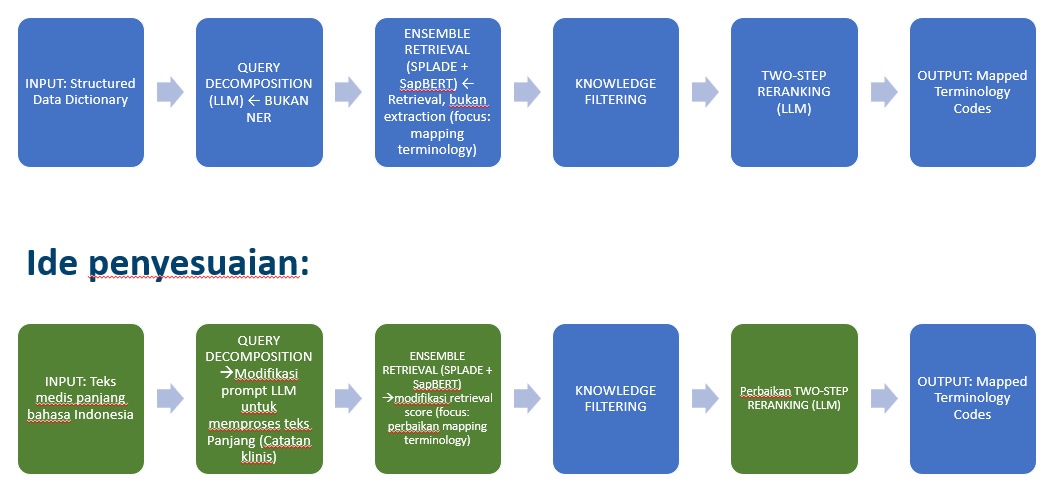
\includegraphics[width=0.9\textwidth]{prism-uploads/image.png}
    \caption{Gambaran arsitektur dan alur \textit{pipeline} yang diusulkan}
    \label{fig:arsitektur-usulan-model}
\end{figure}

\newcounter{algoritma}[chapter]
\renewcommand{\thealgoritma}{\arabic{chapter}.\arabic{algoritma}}

\textit{Pseudo code} pada Algoritma~\ref{alg:pemetaan-terminologi} merangkum alur operasional model dari masukan teks klinis sampai terbentuknya keluaran pemetaan dan pembaruan \textit{knowledge reservoir}.

\par
\begingroup
\scriptsize
\setstretch{1}
\renewcommand{\LTcaptype}{algoritma}
\providecommand{\theHalgoritma}{\theHchapter.\arabic{algoritma}}
\setlength{\tabcolsep}{0pt}
\newcommand{\algtext}[2]{\hspace*{#1em}\parbox[t]{\dimexpr\linewidth-#1em\relax}{\raggedright #2\strut}}
\Needspace{12\baselineskip}
\begin{longtable}{@{}p{1.8em}@{\hspace{0.6em}}p{\dimexpr0.96\textwidth-2.4em\relax}@{}}
\hline
\multicolumn{2}{@{}p{0.96\textwidth}@{}}{\textbf{Algoritma~\thealgoritma. Pemetaan Terminologi Klinis Bahasa Indonesia}\label{alg:pemetaan-terminologi}}\\
\hline
\multicolumn{2}{@{}p{0.96\textwidth}@{}}{\textbf{Masukan:} teks klinis panjang atau daftar istilah RME; basis pengetahuan SNOMED CT, LOINC, ICD-10; \textit{knowledge reservoir}; aturan pemetaan; dan parameter model.}\\
\multicolumn{2}{@{}p{0.96\textwidth}@{}}{\textbf{Keluaran:} hasil pemetaan dan antrean validasi ahli.}\\[0.5em]
\endfirsthead
\hline
\multicolumn{2}{@{}p{0.96\textwidth}@{}}{\textbf{Algoritma~\thealgoritma. Pemetaan Terminologi Klinis Bahasa Indonesia (lanjutan)}}\\
\hline
\endhead
\multicolumn{2}{@{}r@{}}{\textit{Bersambung ke halaman berikutnya.}}\\
\hline
\endfoot
\hline
\endlastfoot
1. & \algtext{0}{$teks\_bersih \leftarrow$ pra-pemrosesan dan normalisasi bahasa($teks\_masukan$)}\\*
2. & \algtext{0}{$daftar\_entitas \leftarrow$ ekstraksi multi-entitas dan metadata ke JSON($teks\_bersih$)}\\*
3. & \algtext{0}{$masukan\_QD \leftarrow$ penerapan \textit{mapping rules} dan transformasi format($daftar\_entitas$)}\\*
4. & \algtext{0}{$daftar\_tugas \leftarrow$ dekomposisi kueri dan penentuan target($masukan\_QD$)}\\*
5. & \algtext{0}{$hasil\_pemetaan \leftarrow \emptyset$; $antrean\_validasi \leftarrow \emptyset$}\\
6. & \algtext{0}{\textbf{for} setiap $tugas$ \textbf{in} $daftar\_tugas$ \textbf{do}}\\*
7. & \algtext{1}{$rekaman \leftarrow$ cari pemetaan pada \textit{knowledge reservoir}($tugas$)}\\
8. & \algtext{1}{\textbf{if} rekaman tervalidasi ahli, sesuai konteks, dan kode masih valid \textbf{then}}\\*
9. & \algtext{2}{$hasil \leftarrow$ pemetaan dari rekaman}\\
10. & \algtext{1}{\textbf{else}}\\*
11. & \algtext{2}{$kandidat\_sparse \leftarrow$ \textit{retrieval} SPLADE($tugas$)}\\*
12. & \algtext{2}{$kandidat\_dense \leftarrow$ \textit{retrieval} SapBERT($tugas$)}\\*
13. & \algtext{2}{$kandidat \leftarrow$ gabungkan skor dan pilih Top-$k$ kandidat (Persamaan~\ref{eq:hybrid-retrieval})}\\
14. & \algtext{2}{$kandidat\_valid \leftarrow$ \textit{filtering} domain, atribut, konsep aktif, dan ambang skor \textit{hybrid}($kandidat$)}\\*
15. & \algtext{2}{$hasil \leftarrow$ \textit{abstain} tanpa kode final}\\
16. & \algtext{2}{\textbf{if} $kandidat\_valid$ tidak kosong \textbf{then}}\\*
17. & \algtext{3}{$penilaian \leftarrow$ \textit{reranking} LLM sebanyak $T$ kali($kandidat\_valid$, $tugas$)}\\*
18. & \algtext{3}{$label, konsistensi \leftarrow$ agregasi hasil penilaian}\\*
19. & \algtext{3}{$skor\_akhir \leftarrow$ normalisasi dan pembobotan enam komponen (Persamaan~\ref{eq:final-mapping-score})}\\*
20. & \algtext{3}{$terbaik \leftarrow$ pilih kandidat dengan skor akhir tertinggi}\\
21. & \algtext{3}{\textbf{if} label terbaik memenuhi syarat relevansi, tidak ada konflik, serta skor dan konsistensi memenuhi ambang (Persamaan~\ref{eq:acceptance-decision}) \textbf{then}}\\*
22. & \algtext{4}{$hasil \leftarrow$ kode terbaik dengan status diterima otomatis}\\*
23. & \algtext{3}{\textbf{end if}}\\
24. & \algtext{3}{lengkapi hasil dengan kandidat, label, dan skor penilaian}\\*
25. & \algtext{2}{\textbf{end if}}\\
26. & \algtext{2}{tambahkan hasil ke $antrean\_validasi$, prioritaskan kasus \textit{abstain}}\\*
27. & \algtext{1}{\textbf{end if}}\\
28. & \algtext{1}{tambahkan hasil beserta entitas asal, target, dan konteks ke $hasil\_pemetaan$}\\*
29. & \algtext{0}{\textbf{end for}}\\*
30. & \algtext{0}{\textbf{return} $hasil\_pemetaan$, $antrean\_validasi$}\\[0.5em]
\multicolumn{2}{@{}p{0.96\textwidth}@{}}{\textbf{Tindak lanjut ketika hasil validasi ahli tersedia:}}\\*
31. & \algtext{0}{\textbf{for} setiap hasil yang telah diperiksa ahli \textbf{do}}\\*
32. & \algtext{1}{perbarui $hasil\_pemetaan$ sesuai persetujuan, koreksi, atau keputusan tidak ada padanan}\\*
33. & \algtext{1}{\textbf{if} pemetaan ke kode valid disahkan ahli \textbf{then}}\\*
34. & \algtext{2}{perbarui \textit{knowledge reservoir} dengan kueri, konteks, target, versi terminologi, kode, dan metadata validasi}\\*
35. & \algtext{1}{\textbf{end if}}\\*
36. & \algtext{0}{\textbf{end for}}\\*[0.5em]
\multicolumn{2}{@{}p{0.96\textwidth}@{}}{\textbf{Catatan:} syarat relevansi pada baris 21 adalah label \textit{exact match} atau \textit{highly relevant}, tanpa seri label. Hasil otomatis dapat dikeluarkan langsung, tetapi hanya hasil yang disahkan ahli yang disimpan ke reservoir.}\\
\end{longtable}
\endgroup

\subsection{Formalisasi Matematis Model Usulan}

Berbeda dari formula umum RAG dan \textit{retrieval} pada Bab III, formula pada bagian ini merupakan operasionalisasi model yang diusulkan dalam penelitian. Formula ini bukan formula asli CDE-Mapper Gilani, melainkan adaptasi yang dirancang agar pemilihan kandidat untuk terminologi klinis Bahasa Indonesia lebih transparan, dapat direplikasi, dan dapat diuji kontribusi tiap komponennya.

Setelah kandidat Top-$k$ diperoleh menggunakan Persamaan~\ref{eq:hybrid-retrieval}, kandidat disaring berdasarkan ambang skor dan kesesuaian terminologi target:

\begin{equation}
C'(q)=\left\{c\in C_k(q)\;\middle|\;
s_{\mathrm{hybrid}}(q,c)\geq\tau_{\mathrm{filter}}
\land d(c)\in D(q)\right\},
\label{eq:candidate-filtering}
\end{equation}

dengan $D(q)$ sebagai himpunan terminologi atau domain yang diizinkan oleh hasil klasifikasi dan \textit{linking rules}, $d(c)$ sebagai domain kandidat, dan $\tau_{\mathrm{filter}}$ sebagai ambang yang ditentukan pada data pengembangan. Penggunaan himpunan $D(q)$ memungkinkan lebih dari satu terminologi tetap dipertimbangkan ketika klasifikasi domain belum pasti. Skor atribut dihitung dari proporsi atribut hasil dekomposisi yang dipertahankan kandidat:

\begin{equation}
S_{\mathrm{atribut}}(q,c)=
\frac{|A(q)\cap A(c)|}{\max\{1,|A(q)|\}},
\label{eq:attribute-coverage-score}
\end{equation}

dengan $A(q)$ sebagai atribut klinis pada kueri, misalnya lokasi anatomis, spesimen, metode, waktu, satuan, posisi tubuh, atau tingkat keparahan, dan $A(c)$ sebagai atribut yang tercakup oleh kandidat.

Kesesuaian domain kandidat dihitung menggunakan probabilitas yang dihasilkan pengklasifikasi atau modul \textit{routing}:

\begin{equation}
S_{\mathrm{domain}}(q,c)=p\!\left(d(c)\mid q\right),
\label{eq:domain-compatibility-score}
\end{equation}

sehingga kandidat dari domain yang masih diizinkan dapat memiliki tingkat kecocokan yang berbeda. Kesesuaian granularitas dihitung dari jarak antara tingkat kekhususan yang diharapkan untuk kueri dan tingkat kekhususan kandidat:

\begin{equation}
S_{\mathrm{granularitas}}(q,c)=
\exp\!\left(-\frac{|g(q)-g(c)|}{\rho}\right),
\label{eq:granularity-score}
\end{equation}

dengan $g(q),g(c)\in[0,1]$ sebagai tingkat kekhususan yang dinormalisasi menurut hierarki atau atribut terminologi target dan $\rho>0$ sebagai parameter toleransi. Definisi operasional $g$ disusun bersama ahli dan ditetapkan sebelum pengujian.

Kestabilan \textit{reranking} LLM diukur menggunakan proporsi keputusan mayoritas dari $T$ pengulangan:

\begin{equation}
S_{\mathrm{konsistensi}}(q,c)=
\max_{\ell\in\mathcal{L}}
\frac{1}{T}\sum_{t=1}^{T}
\mathbf{1}\!\left(L^{(t)}(q,c)=\ell\right),
\label{eq:reranking-self-consistency}
\end{equation}

dengan $\mathcal{L}$ sebagai himpunan label relevansi. Pengambilan keputusan mayoritas ini mengadaptasi prinsip \textit{self-consistency}, yaitu mengagregasi beberapa jalur keluaran untuk memperoleh keputusan yang lebih stabil \citep{wang_self-consistency_2023}. Karena skor berasal dari komponen yang berbeda, setiap komponen $S_j$ dinormalisasi pada himpunan kandidat suatu kueri:

\begin{equation}
\widetilde{S}_{j}(q,c)=
\frac{S_j(q,c)-\min_{c'\in C'(q)}S_j(q,c')}
{\max_{c'\in C'(q)}S_j(q,c')-\min_{c'\in C'(q)}S_j(q,c')+\varepsilon},
\label{eq:score-normalization}
\end{equation}

dengan $\varepsilon$ sebagai konstanta kecil untuk mencegah pembagian dengan nol. Skor akhir kandidat kemudian menggabungkan enam bukti yang telah dinormalisasi:

\begin{equation}
\begin{split}
S_{\mathrm{akhir}}(q,c)={}&
w_l\widetilde{S}_{\mathrm{leksikal}}(q,c)
+w_s\widetilde{S}_{\mathrm{semantik}}(q,c)
+w_d\widetilde{S}_{\mathrm{domain}}(q,c)\\
&+w_a\widetilde{S}_{\mathrm{atribut}}(q,c)
+w_g\widetilde{S}_{\mathrm{granularitas}}(q,c)
+w_k\widetilde{S}_{\mathrm{konsistensi}}(q,c),
\end{split}
\label{eq:final-mapping-score}
\end{equation}

dengan kendala:

\begin{equation}
w_l+w_s+w_d+w_a+w_g+w_k=1,
\qquad w_i\geq0.
\label{eq:score-weight-constraint}
\end{equation}

$S_{\mathrm{leksikal}}$ berasal dari SPLADE \citep{formal_splade_2021}; $S_{\mathrm{semantik}}$ berasal dari SapBERT \citep{liu_self-alignment_2021}; $S_{\mathrm{domain}}$ menunjukkan keyakinan modul \textit{routing} terhadap terminologi kandidat; $S_{\mathrm{atribut}}$ menunjukkan kelengkapan atribut; $S_{\mathrm{granularitas}}$ menunjukkan kesesuaian tingkat kekhususan konsep; dan $S_{\mathrm{konsistensi}}$ menunjukkan kestabilan keputusan LLM. Bobot awal ditetapkan sama, kemudian dipilih melalui \textit{grid search} pada data pengembangan dengan Accuracy@1 sebagai sasaran utama dan \textit{coverage} sebagai kendala tambahan. Data uji tidak digunakan untuk menentukan bobot atau ambang.

Kandidat terbaik adalah $c^*=\operatorname*{arg\,max}_{c\in C'(q)}S_{\mathrm{akhir}}(q,c)$. Untuk mencegah pemetaan yang dipaksakan, keputusan akhir menggunakan mekanisme \textit{abstain}:

\begin{equation}
\widehat{c}(q)=
\begin{cases}
c^*, & S_{\mathrm{akhir}}(q,c^*)\geq\tau_{\mathrm{accept}}
\land S_{\mathrm{konsistensi}}(q,c^*)\geq\delta,\\
\varnothing, & \text{selainnya},
\end{cases}
\label{eq:acceptance-decision}
\end{equation}

dengan $\varnothing$ berarti kasus dikirim untuk validasi ahli. Nilai $\tau_{\mathrm{accept}}$ dan $\delta$ ditentukan pada data pengembangan dengan mempertimbangkan pertukaran antara akurasi dan \textit{coverage}.


\subsection{Asumsi, Batasan, dan Strategi Mitigasi}

Model mengasumsikan akses terhadap terminologi standar yang relevan dan/atau ekspor terminologi dari SATUSEHAT, serta ketersediaan sampel data klinis yang dapat dianonimkan untuk pengembangan dan evaluasi. Batasan utama meliputi: (1) variasi bahasa yang sangat ekstrem pada catatan klinis, (2) konsep lokal yang tidak memiliki padanan langsung pada terminologi target, (3) potensi halusinasi pada LLM saat ekstraksi atau \textit{reranking}, serta (4) kebutuhan validasi ahli. Untuk mitigasi, penelitian mengusulkan penggunaan \textit{constraint} terminologi pada tahap \textit{filtering}, penerapan \textit{threshold} dan \textit{self-consistency} pada \textit{reranking}, serta penerapan \textit{human-in-the-loop} dan \textit{knowledge reservoir} untuk meningkatkan kualitas secara iteratif.

\section{Rancangan Pengujian}

Bagian ini menjelaskan rancangan pengujian untuk mengevaluasi performa model usulan pada tugas pemetaan terminologi klinis Bahasa Indonesia ke SNOMED CT, LOINC, dan ICD-10. Rancangan dibuat untuk mengukur akurasi pemetaan, ketahanan terhadap variasi bahasa, kontribusi setiap komponen (\textit{ablation}), serta kesiapan penerapan pada konteks interoperabilitas SATUSEHAT.

\subsection{Desain Eksperimen dan Skenario Pengujian}

\begin{enumerate}
    \item \textbf{\textit{Terminology mapping} dari istilah pendek (\textit{single-mention}).} \textit{Input} berupa daftar istilah atau \textit{field} dari kamus data RME atau label klinis singkat. Tujuannya adalah mengukur kemampuan normalisasi istilah lokal dan varian ejaan.
    \item \textbf{\textit{End-to-end mapping} dari teks panjang (\textit{multi-mention}).} \textit{Input} berupa dokumen klinis panjang berbahasa Indonesia. Tujuannya adalah mengukur \textit{pipeline} lengkap, yaitu ekstraksi dan \textit{mapping}, serta dampak \textit{error propagation}.
    \item \textbf{\textit{Multi-terminology routing}.} Pengujian ini menilai kemampuan sistem memilih terminologi target yang tepat, yaitu SNOMED CT, LOINC, atau ICD-10, berdasarkan tipe entitas dan konteks \citep{ayuningtyas_bringing_2025}.
    \item \textbf{\textit{Robustness} terhadap variasi bahasa.} Pengujian dilakukan pada subset data yang mengandung singkatan, campuran bahasa Indonesia--Inggris, istilah lokal, dan \textit{typo} \citep{purwitasari_comparison_2023}.
\end{enumerate}

\subsection{Dataset, Pembagian Data, dan \textit{Gold Standard}}

Dataset evaluasi dibangun dari sampel istilah dan/atau dokumen yang merepresentasikan data klinis Indonesia, kemudian dianotasi menjadi \textit{gold standard} oleh ahli. Untuk memastikan evaluasi yang adil, data dipisahkan menjadi: (i) data pengembangan untuk \textit{tuning threshold}, bobot skor, \textit{prompt}, aturan, dan konfigurasi \textit{retriever}; serta (ii) data uji (\textit{hold-out}) yang tidak digunakan selama pengembangan.

\subsubsection{Data untuk Pengembangan Model}

Untuk keperluan pengembangan model, penelitian ini menggunakan data istilah klinis dalam bahasa Indonesia yang dikumpulkan dari empat sumber utama.

\begin{enumerate}
    \item Data terminologi medis standar, yaitu SNOMED CT, LOINC, dan ICD-10, yang diakses dari SATUSEHAT dan sumber terminologi observasional terbuka yang relevan.
    \item Kamus data elektronik rekam medis (RME) lokal yang diperoleh dari sampel rumah sakit atau puskesmas di Indonesia yang telah menerapkan RME. Data ini mencakup istilah diagnosis, prosedur, observasi, dan obat-obatan dalam format asli sesuai entri tenaga kesehatan.
    \item Dataset dari penelitian Gilani, seperti NCBI Corpus dan BC5CDR, untuk mendukung pengembangan awal dan pengujian komponen tertentu \citep{gilani_cde-mapper_2025}.
    \item Platform konsultasi kesehatan daring. Data anonim dari sesi tanya jawab tentang kesehatan dikumpulkan untuk mendapatkan representasi bahasa sehari-hari pasien, termasuk variasi istilah, singkatan informal, dan kesalahan ejaan. Data ini penting untuk menguji ketahanan model terhadap variasi leksikal di dunia nyata \citep{purwitasari_comparison_2023}.
\end{enumerate}

\subsubsection{Data untuk Evaluasi}

Untuk keperluan evaluasi yang valid, sebuah dataset \textit{gold standard} dikembangkan dengan melibatkan tenaga medis, seperti dokter atau perekam medis. Prosesnya meliputi:

\begin{enumerate}
    \item \textbf{Seleksi sampel.} Memilih sampel istilah dari data sumber, misalnya 100--200 istilah, yang mewakili variasi tantangan, seperti istilah standar, singkatan, dan kesalahan eja.
    \item \textbf{Anotasi manual.} Minimal dua anotator, misalnya dokter dan/atau perekam medis, melakukan pemetaan secara terpisah. Selain kode benar, anotasi mencakup domain entitas, terminologi target, atribut klinis yang harus dipertahankan, tingkat kekhususan yang diharapkan, dan keputusan apakah kasus dapat dipetakan otomatis atau memerlukan tinjauan ahli.
    \item \textbf{Validasi antar-anotator.} Tingkat kesepakatan antar-anotator dihitung untuk memastikan kualitas dan konsistensi dataset \textit{gold standard}. Perbedaan diselesaikan melalui adjudikasi oleh ahli ketiga sebelum data digunakan untuk evaluasi.
\end{enumerate}

\subsection{\textit{Baseline}, Model Pembanding, dan Varian (\textit{Ablation Study})}

Evaluasi dibagi menjadi perbandingan dengan \textit{baseline} dan pengujian varian \textit{ablation}. Perbandingan modul pemetaan menggunakan masukan entitas atau CDE yang sama agar perbedaan kemampuan ekstraksi tidak tercampur dengan kualitas pemetaan. Evaluasi \textit{end-to-end} pada teks panjang dilaporkan secara terpisah.

\subsubsection{Baseline Pembanding}

\begin{enumerate}
    \item \textbf{Pencocokan leksikal.} Pemetaan pada label dan sinonim terminologi menggunakan dua konfigurasi, yaitu \textit{exact matching} setelah normalisasi sederhana dan \textit{fuzzy matching} berdasarkan kemiripan string. Keduanya menjadi pembanding untuk menilai kemampuan metode sederhana dalam menangani istilah baku dan variasi ejaan.
    \item \textbf{LLM \textit{zero-shot} tanpa RAG.} LLM diminta menentukan kode terminologi tanpa contoh pemetaan dan tanpa akses \textit{retrieval}. Untuk mengukur kontribusi penambahan konteks hasil \textit{retrieval}, digunakan pasangan konfigurasi dengan dan tanpa RAG yang memakai model serta versi LLM yang sama, dengan masukan, instruksi tugas, dan format keluaran yang sebanding. Evaluasi mencakup akurasi dan proporsi kode keluaran yang tidak tersedia dalam versi terminologi yang digunakan.
    \item \textbf{CDE-Mapper asli.} Arsitektur CDE-Mapper \citep{gilani_cde-mapper_2025} tanpa adaptasi khusus bahasa Indonesia digunakan sebagai pembanding utama sesuai ketersediaan implementasi dan sumber daya. Pengujian \textit{cross-lingual} dilakukan dengan memberikan CDE berbahasa Indonesia secara langsung. Jika memungkinkan, ditambahkan konfigurasi penerjemahan CDE ke bahasa Inggris sebelum pemetaan. Seluruh konfigurasi diuji pada kasus dan padanan kode yang sama; perubahan konfigurasi yang diperlukan serta keterbatasan replikasi dilaporkan secara eksplisit.
\end{enumerate}

\subsubsection{Ablation Study}

Setiap varian dibandingkan dengan model lengkap dengan menonaktifkan satu komponen yang ditentukan, sementara komponen lain dipertahankan. Lima varian yang diuji adalah sebagai berikut.

\begin{enumerate}
    \item \textbf{Tanpa \textit{preprocessing} khusus bahasa Indonesia.} Normalisasi singkatan medis dan \textit{stemming} dinonaktifkan, sedangkan pembersihan teknis dan segmentasi kalimat tetap digunakan. Varian ini menilai kontribusi kedua proses tersebut, khususnya pada subset istilah lokal dan singkatan.
    \item \textbf{Tanpa \textit{knowledge filtering}.} Kandidat Top-\textit{k} diteruskan ke tahap \textit{reranking} tanpa penyaringan pasca-\textit{retrieval} berdasarkan domain, atribut, dan ambang skor. Basis terminologi, pembatasan konsep aktif pada indeks, dan aturan \textit{routing} tetap sama. Varian ini mengukur kontribusi penyaringan kandidat terhadap akurasi dan cakupan pemetaan.
    \item \textbf{Tanpa \textit{reranking} berbasis LLM.} Penilaian ulang kandidat oleh LLM beserta agregasi label dan skor konsistensinya dinonaktifkan. Kandidat akhir dipilih berdasarkan skor \textit{hybrid retrieval} setelah \textit{filtering}, dengan ambang penerimaan yang ditetapkan pada data pengembangan. Penggunaan LLM pada komponen lain tetap dipertahankan sehingga varian ini secara khusus menilai kontribusi tahap \textit{reranking}, bukan seluruh penggunaan LLM.
    \item \textbf{Tanpa pemanfaatan \textit{cache knowledge reservoir}.} Pengambilan langsung hasil pemetaan terdahulu dinonaktifkan sehingga setiap kueri menjalani proses pencarian dan penilaian kandidat. Contoh pemetaan untuk komponen lain dipertahankan tetap sama. Efisiensi dibandingkan pada kondisi \textit{cold cache} dan \textit{warm cache} melalui waktu inferensi, jumlah panggilan LLM, penggunaan token, dan tingkat \textit{cache hit}, disertai pemeriksaan akurasi. Reservoir tidak diisi dengan jawaban \textit{gold standard} data uji; sumber pemetaan tervalidasi dan urutan kueri untuk pengujian cache ditetapkan sebelumnya.
    \item \textbf{Tanpa \textit{routing} terminologi sebelum pencarian.} Pencarian dilakukan pada gabungan SNOMED CT, LOINC, dan ICD-10 tanpa pembatasan awal berdasarkan domain entitas. Konfigurasi ini dibandingkan dengan pencarian terarah pada terminologi hasil \textit{routing}, sementara basis terminologi, jumlah kandidat Top-\textit{k}, dan penyaringan pasca-\textit{retrieval} tetap sama. Evaluasi menilai presisi, Recall@\textit{k}, dan ketepatan terminologi keluaran untuk mengetahui dampak pembatasan ruang pencarian.
\end{enumerate}

Seluruh perbandingan menggunakan pembagian data uji yang sama dan versi terminologi yang terdokumentasi. Konfigurasi kamus, sinonim, model, serta parameter dicatat untuk menjaga keterbandingan. Penyesuaian ambang atau aturan keputusan yang diperlukan ketika suatu komponen dinonaktifkan hanya menggunakan data pengembangan. Pada pengujian ablation selain cache, penggunaan ulang hasil pemetaan dinonaktifkan secara seragam pada model lengkap dan variannya agar komponen yang diuji benar-benar dijalankan.

\subsection{Metrik Evaluasi}

Metrik evaluasi pada penelitian ini dirancang untuk mengukur performa \textit{framework} secara komprehensif pada dua tingkat, yaitu tingkat pemetaan kandidat kode dan tingkat performa \textit{end-to-end} dari ekstraksi hingga normalisasi konsep. Pemilihan metrik ini mengikuti praktik evaluasi pada tugas \textit{clinical concept normalization}, \textit{ontology alignment}, dan \textit{retrieval-augmented terminology mapping}, yang menekankan ketepatan kandidat teratas, ketercakupan kandidat benar dalam Top-\textit{k}, keseimbangan antara ketepatan dan kelengkapan ekstraksi, serta efisiensi inferensi \citep{chen_clinical_2020,he_bertmap_2022,gilani_cde-mapper_2025,park_development_2026,yu_large_2026}. Definisi konseptual dan persamaan matematis untuk metrik-metrik tersebut telah dibahas pada Bab III, sehingga pada bagian ini rumus tidak dituliskan ulang, tetapi direferensikan sesuai label persamaan yang tersedia.

\begin{enumerate}
    \item \textbf{Accuracy@1.} Untuk mengevaluasi ketepatan kandidat teratas, penelitian ini menggunakan metrik akurasi sebagaimana didefinisikan pada Persamaan~\ref{eq:accuracy}. Pada implementasinya, akurasi digunakan untuk menilai proporsi pemetaan yang benar pada kandidat utama yang dipilih sistem \citep{chen_clinical_2020,gilani_cde-mapper_2025}.

    \item \textbf{Accuracy@\textit{k}.} Untuk menilai apakah kode \textit{gold standard} muncul di dalam himpunan Top-\textit{k} kandidat, penelitian ini menggunakan metrik \textit{Top-k accuracy} sebagaimana dinyatakan pada Persamaan~\ref{eq:topk}. Metrik ini relevan karena pada skenario \textit{retrieval} kandidat benar tidak selalu berada pada peringkat pertama, tetapi tetap perlu muncul dalam daftar kandidat teratas untuk ditinjau lebih lanjut \citep{he_bertmap_2022,gilani_cde-mapper_2025,park_development_2026}.

    \item \textbf{MRR dan Recall@\textit{k}.} MRR pada Persamaan~\ref{eq:mrr} digunakan untuk menilai seberapa awal kandidat benar muncul, sedangkan Recall@\textit{k} pada Persamaan~\ref{eq:recallatk} digunakan ketika satu kueri memiliki lebih dari satu konsep relevan.

    \item \textbf{Precision, Recall, dan F1-score.} Untuk skenario \textit{end-to-end} pada teks panjang, ketika sistem harus mengekstraksi entitas klinis sekaligus memetakannya ke terminologi target, penelitian ini menggunakan \textit{precision}, \textit{recall}, dan F1-score yang masing-masing dirumuskan pada Persamaan~\ref{eq:precision}, Persamaan~\ref{eq:recall}, dan Persamaan~\ref{eq:f1score}. Ketiga metrik ini digunakan untuk menilai keseimbangan antara ketepatan prediksi, kelengkapan temuan entitas, dan performa keseluruhan sistem \citep{chen_clinical_2020}.

    \item \textbf{Coverage.} Untuk mengetahui sejauh mana sistem mampu memberikan setidaknya satu kandidat kode valid setelah tahap \textit{retrieval} dan \textit{filtering}, penelitian ini menggunakan metrik \textit{coverage} sebagaimana didefinisikan pada Persamaan~\ref{eq:coverage}. Metrik ini penting karena sistem yang tampak akurat pada kasus tertentu belum tentu memiliki keluasan cakupan yang baik terhadap seluruh data masukan \citep{gilani_cde-mapper_2025,park_development_2026}.

    \item \textbf{Agreement atau consistency.} Untuk menilai kestabilan keputusan sistem, penelitian ini menggunakan dua ukuran yang saling melengkapi, yaitu konsistensi hasil \textit{reranking} sebagaimana dirumuskan pada Persamaan~\ref{eq:consistency} dan koefisien Kappa untuk kesepakatan antar-anotator sebagaimana dinyatakan pada Persamaan~\ref{eq:kappa}. Penggunaan dua ukuran ini penting karena penelitian memerlukan \textit{gold standard} yang andal sekaligus sistem yang stabil ketika dihadapkan pada istilah atau dokumen yang serupa \citep{januel_improved_2011,gilani_cde-mapper_2025}.

    \item \textbf{Efisiensi.} Selain akurasi, penelitian ini juga mengukur efisiensi komputasi melalui rata-rata waktu inferensi sebagaimana dirumuskan pada Persamaan~\ref{eq:efficiency-time}. Untuk membandingkan peningkatan efisiensi terhadap metode pembanding, digunakan pula persentase percepatan sebagaimana dinyatakan pada Persamaan~\ref{eq:speedup}. Kedua ukuran ini diperlukan agar model yang diusulkan tidak hanya akurat, tetapi juga layak diterapkan pada skenario penggunaan praktis \citep{gilani_cde-mapper_2025,park_development_2026}.

    \item \textbf{Pertukaran akurasi--\textit{coverage}.} Mekanisme \textit{abstain} dievaluasi pada beberapa nilai $\tau_{\mathrm{accept}}$ dan $\delta$. Analisis ini menunjukkan perubahan akurasi pada kasus yang diterima ketika proporsi kasus yang dipetakan otomatis dinaikkan atau diturunkan.
\end{enumerate}

Melalui kombinasi metrik tersebut, evaluasi pada penelitian ini tidak hanya menilai apakah sistem menghasilkan kode yang benar, tetapi juga menilai kemampuan sistem menyediakan kandidat yang relevan, mengekstraksi entitas secara lengkap, mempertahankan konsistensi hasil, dan bekerja secara efisien pada skenario penggunaan nyata.

\subsection{Prosedur Pengujian dan Analisis Hasil}

\begin{enumerate}
    \item \textbf{Konfigurasi.} Menetapkan variasi model, yaitu \textit{baseline} versus usulan, parameter \textit{retrieval} (Top-\textit{k}), bobot skor, \textit{threshold filtering}, ambang penerimaan, jumlah pengulangan LLM, dan \textit{prompt} atau format \textit{output} untuk LLM. Seluruh parameter dipilih hanya dari data pengembangan.
    \item \textbf{Eksekusi pada data uji.} Menjalankan seluruh model pada dataset uji dan menyimpan \textit{output} terstruktur, yaitu kandidat, skor, keputusan, dan log komponen.
    \item \textbf{Perhitungan metrik.} Menghitung Accuracy@1, Accuracy@\textit{k}, Recall@\textit{k}, MRR, Precision, Recall, F1, \textit{coverage}, konsistensi, dan efisiensi komputasi.
    \item \textbf{\textit{Ablation} dan uji sensitivitas.} Menjalankan varian \textit{ablation} untuk mengukur kontribusi modul dan komponen skor, serta menguji sensitivitas terhadap bobot, Top-\textit{k}, $\tau_{\mathrm{filter}}$, $\tau_{\mathrm{accept}}$, $\delta$, dan jumlah pengulangan LLM.
    \item \textbf{\textit{Error analysis}.} Mengelompokkan kesalahan menjadi: (a) \textit{error} ekstraksi, yaitu entitas terlewat atau salah tipe; (b) \textit{error retrieval}, yaitu kandidat benar tidak muncul; (c) \textit{error filtering}, yaitu kandidat benar ditemukan tetapi dibuang; (d) \textit{error reranking}, yaitu kandidat benar ada tetapi tidak dipilih; (e) \textit{abstention error}, yaitu kasus yang sebenarnya dapat dipetakan tetapi ditolak; (f) \textit{overconfident error}, yaitu kandidat salah diterima dengan skor tinggi; (g) \textit{error} terminologi, yaitu tidak ada padanan; dan (h) \textit{error} bahasa, seperti singkatan, \textit{typo}, atau ambiguitas. Hasil analisis digunakan untuk menyusun rekomendasi perbaikan iteratif pada komponen dan \textit{guideline} anotasi.
\end{enumerate}

\section{Jadwal Penelitian}

Tahapan kegiatan penelitian dan rencana jadwal pelaksanaan untuk setiap tahapan kegiatan dalam penelitian ini, yang difokuskan pada Tahun II dan Tahun III, secara ringkas ditunjukkan pada Tabel~\ref{tab:jadwal-penelitian}.


\begin{table}[H]
\centering
\caption{Rencana jadwal pelaksanaan kegiatan penelitian}
\label{tab:jadwal-penelitian}
\scriptsize
\setlength{\tabcolsep}{3pt}
\renewcommand{\arraystretch}{1.15}
\resizebox{\textwidth}{!}{%
\begin{tabular}{>{\raggedright\arraybackslash}p{4.4cm} *{8}{c} >{\raggedright\arraybackslash}p{6.1cm}}
\toprule
\textbf{Jenis Kegiatan} & \multicolumn{4}{c}{\textbf{Tahun II}} & \multicolumn{4}{c}{\textbf{Tahun III}} & \textbf{Indikator} \\
\cmidrule(lr){2-5} \cmidrule(lr){6-9}
& \textbf{1} & \textbf{2} & \textbf{3} & \textbf{4} & \textbf{1} & \textbf{2} & \textbf{3} & \textbf{4} & \\
\midrule
\textbf{Tahap I} & & & & & & & & & \\
\midrule
Kajian teori dan studi pustaka & $\checkmark$ & $\checkmark$ & $\checkmark$ & $\checkmark$ & & & & & Diperbaruinya referensi sebagai penunjang tinjauan pustaka \\
\midrule
Menentukan \textit{roadmap} penelitian & $\checkmark$ & $\checkmark$ & & & & & & & \textit{Roadmap} penelitian dan draf proposal \\
\midrule
Ujian proposal & & & $\checkmark$ & & & & & & Ujian pra-komprehensif dan komprehensif \\
\midrule
Revisi proposal & & & & $\checkmark$ & & & & & Proposal yang telah direvisi dan ditandatangani tim penguji \\
\midrule
\textbf{Tahap II} & & & & & & & & & \\
\midrule
Adaptasi model CDE-Mapper & & & $\checkmark$ & $\checkmark$ & $\checkmark$ & & & & Terbentuknya model dan prototipe CDE-Mapper untuk teks klinis panjang; naskah publikasi \\
\midrule
Pembangunan dataset & & & $\checkmark$ & $\checkmark$ & $\checkmark$ & & & & Dataset untuk pengujian dan pelatihan model siap digunakan \\
\midrule
Implementasi \textit{preprocessing} teks klinis & & & & $\checkmark$ & $\checkmark$ & $\checkmark$ & & & Terbentuknya model untuk \textit{preprocessing} teks klinis panjang dalam bahasa Indonesia \\
\midrule
Implementasi inti model & & & & & $\checkmark$ & $\checkmark$ & & & Terbentuknya model adaptasi CDE-Mapper \\
\midrule
Pengujian model & & & & & & $\checkmark$ & $\checkmark$ & & Pengujian model pada berbagai skenario uji; naskah publikasi \\
\midrule
Pembuatan laporan akhir dan persiapan ujian tertutup & & & & & & $\checkmark$ & $\checkmark$ & & Draf laporan disertasi \\
\midrule
\textbf{Tahap III} & & & & & & & & & \\
\midrule
Penilaian dan kelayakan disertasi & & & & & & & $\checkmark$ & & Laporan disertasi layak untuk diujikan \\
\midrule
Ujian tertutup & & & & & & & $\checkmark$ & & Terlaksananya ujian tertutup \\
\midrule
Revisi hasil ujian tertutup & & & & & & & & $\checkmark$ & Laporan disertasi disetujui oleh tim penguji \\
\bottomrule
\end{tabular}%
}
\normalsize
\end{table}

% Daftar Pustaka
\addcontentsline{toc}{chapter}{DAFTAR PUSTAKA}
\bibliography{term-mapping}

\end{document}